%%%% IACR Transactions TEMPLATE %%%%
% This file shows how to use the iacrtrans class to write a paper.
% Written by Gaetan Leurent gaetan.leurent@inria.fr (2020)
% Public Domain (CC0)

%%%% 1. DOCUMENTCLASS %%%%
\documentclass[journal=tches,final]{iacrtrans}
%%%% NOTES:
% - Change "journal=tosc" to "journal=tches" if needed
% - Change "submission" to "final" for final version
% - Add "spthm" for LNCS-like theorems

%%%% 2. ALGORITHM PACKAGES %%%%
\usepackage{algorithm}
\usepackage{algorithmic}

%%%% TIKZ PACKAGES FOR FIGURES %%%%
\usepackage{tikz}
\usetikzlibrary{positioning}       % relative positioning
\usetikzlibrary{shapes.geometric}  % shapes like diamond, ellipse
\usetikzlibrary{arrows.meta}       % modern arrow tips
\usetikzlibrary{fit}               % fitting nodes around others
\usetikzlibrary{backgrounds}       % background layers
\usetikzlibrary{calc}              % coordinate calculations
\usetikzlibrary{decorations.pathreplacing}  % braces for annotations

%%%% COLOR PACKAGE FOR HIGHLIGHTING %%%%
\usepackage{xcolor}
\usepackage[normalem]{ulem}  % For wavy underline
% \newcommand{\bluet}[1]{\textcolor{blue}{\uwave{#1}}}
\newcommand{\bluet}[1]{\textcolor{blue}{#1}}

%%%% ALGORITHM GLOBAL SETTINGS %%%%
% Custom commands for consistent Input/Output formatting
\newcommand{\Input}[1]{\STATE \textbf{Input:} #1}
\newcommand{\Output}[1]{\STATE \textbf{Output:} #1}

% Optional: Customize algorithm appearance
\renewcommand{\algorithmicrequire}{\textbf{Input:}}
\renewcommand{\algorithmicensure}{\textbf{Output:}}

%%%% 3. AUTHOR, INSTITUTE %%%%
\author{Jiahao Xiang\inst{1} \and Lang Li\inst{1}}
\institute{
  Hengyang Normal University,  Hengyang, China
  % \and
  % Institute B, City, Country, \email{john@institute}
}
%%%% NOTES:
% - We need a city name for indexation purpose, even if it is redundant
%   (eg: University of Atlantis, Atlantis, Atlantis)
% - \inst{} can be omitted if there is a single institute,
%   or exactly one institute per author

%%%% 4. TITLE %%%%
\title[ML-DSA Digital Signatures in Resource-Constrained MQTT Environments]{ML-DSA Digital Signatures in Resource-Constrained MQTT Environments}
%%%% NOTES:
% - If the title is too long, or includes special macro, please
%   provide a "running title" as optional argument: \title[Short]{Long}
% - You can provide an optional subtitle with \subtitle.

\begin{document}

\maketitle

%%%% 5. KEYWORDS %%%%
\keywords{Post-Quantum Cryptography \and ML-DSA \and MQTT Protocol \and IoT Security \and Resource-Constrained Devices}

%%%% 6. ABSTRACT %%%%
\begin{abstract}
	Large-scale quantum computers necessitate migration of Internet of Things (IoT) systems to post-quantum cryptographic standards. While NIST has standardized ML-DSA (Module-Lattice-Based Digital Signature Algorithm) for digital signatures, practical deployment of post-quantum authentication in resource-constrained IoT environments remains inadequately characterized. ML-DSA integration within MQTT-based IoT systems is evaluated through comprehensive performance analysis on ARM Cortex-M4 microcontrollers. The methodology encompasses signature generation and verification benchmarking, memory utilization analysis, and protocol overhead assessment under realistic IoT constraints. Performance implications of ML-DSA deployment are examined through comparison with classical signature schemes, quantifying computational overhead, memory requirements, and verification latency on resource-constrained devices. These findings reveal fundamental trade-offs between post-quantum security and IoT performance requirements, providing critical insights for practical deployment strategies in resource-limited environments.
\end{abstract}

%%%% 7. PAPER CONTENT %%%%
\section{Introduction}

The emergence of quantum computing fundamentally undermines current cryptographic infrastructures, necessitating systematic migration to post-quantum cryptographic standards across all computing domains~\cite{Khalid2019}. The National Institute of Standards and Technology (NIST) has formalized ML-DSA (Module-Lattice-Based Digital Signature Algorithm) within FIPS 204~\cite{NIST-FIPS-204}, establishing this CRYSTALS-Dilithium-based scheme as the primary standard for post-quantum digital signatures.

The transition from theoretical post-quantum standardization to practical deployment has revealed fundamental implementation challenges extending beyond algorithmic considerations~\cite{MLDSAHardware2024}. Post-quantum signature schemes impose substantial computational and storage overhead compared to classical alternatives. ML-DSA signatures span 2,420-4,627 bytes across security levels, representing 30-70× size increases relative to 64-byte ECDSA signatures. These expanded signature sizes, combined with elevated computational demands, substantially exceed the computational and memory capabilities of resource-constrained devices~\cite{HwangKim2024}.

Internet of Things (IoT) systems exemplify these deployment challenges, where computational, memory, and energy limitations constrain cryptographic implementation choices~\cite{Ghosh2019}. Despite performance overhead, signature-based authentication remains essential for applications requiring cryptographic non-repudiation, audit trails, and public key infrastructure compatibility. The MQTT protocol, widely adopted for IoT messaging due to its lightweight design, experiences performance degradation when post-quantum signatures introduce overhead on resource-constrained devices. This disparity between standardization progress and deployment feasibility motivates systematic performance characterization.

\bluet{This work addresses ML-DSA integration within MQTT-based IoT systems through performance analysis on ARM Cortex-M4 microcontrollers. Three contributions advance post-quantum IoT deployment:}

\begin{itemize}
	\item \textbf{Computational Performance Benchmarking}: \bluet{Cycle-accurate measurements of ML-DSA signature operations on ARM Cortex-M4 microcontrollers at 168 MHz, quantifying execution latency and throughput across all three standardized parameter sets.}

	\item \textbf{Memory Utilization Analysis}: \bluet{Static and dynamic memory profiling measuring Flash storage requirements, stack consumption, and peak SRAM utilization during signature operations.}

	\item \textbf{Protocol-Level MQTT Integration Assessment}: \bluet{End-to-end latency and message size overhead evaluation within MQTT publish-subscribe workflows, comparing ML-DSA against ECDSA P-256 baseline.}
\end{itemize}

\bluet{These contributions quantify trade-offs between post-quantum security levels and IoT performance requirements, enabling informed deployment decisions for resource-limited environments.}

The remainder of this paper is organized as follows: Section~\ref{sec:related} presents background information on post-quantum cryptography and related work in IoT deployments. Section~\ref{sec:mldsa} provides an overview of the ML-DSA algorithm and its implementation considerations. Section~\ref{sec:architecture} describes the implementation architecture for MQTT-based IoT systems. Section~\ref{sec:methodology} details the experimental methodology for performance evaluation on ARM Cortex-M4 microcontrollers. Section~\ref{sec:results} presents and analyzes experimental results, examining the trade-offs between security and performance. Finally, Section~\ref{sec:conclusion} concludes with implications for practical deployment and future research directions.

\section{Related Work and Motivation}\label{sec:related}

Conventional network protocols have undergone post-quantum migration analysis~\cite{Kampanakis2020, Sikeridis2020}, yet \bluet{IoT-specific communication protocols remain underexplored}, creating deployment barriers in resource-constrained environments.

\subsection{ML-DSA Performance Benchmarks on Embedded Systems}

Banegas et al.~\cite{Banegas2021} benchmarked CRYSTALS-Dilithium on embedded systems, reporting 1.45$\times$ computational cycles relative to ECDSA on ARM Cortex-M4 processors. This overhead, combined with memory constraints, creates deployment bottlenecks in IoT environments.

The pqm4 benchmarking campaign~\cite{pqm4-benchmarks} extends these observations to standardized ML-DSA parameter sets, reporting tens of kilobytes memory consumption and millions of CPU cycles per signature on Cortex-M4 targets. Measurements on Cortex-M7 microcontrollers~\cite{Benchmark2022} demonstrate reduced latency but maintain signature operations in the tens-of-milliseconds regime, positioning ML-DSA at the threshold of acceptable responsiveness for interactive workloads.

\subsection{Deployment Bottlenecks in IoT Applications}

Practical deployment scenarios reveal performance bottlenecks challenging IoT system viability. Analysis of the SUIT (Software Update for the Internet of Things) framework demonstrates post-quantum signature verification requiring up to 3.2 seconds on low-power microcontrollers, exceeding sub-second latency constraints for real-time IoT applications.

Security vulnerabilities and throughput limitations compound these constraints. Marchsreiter~\cite{Marchsreiter2024} reports order-of-magnitude transaction throughput reductions on embedded blockchain nodes with ML-DSA, where signing latency dominates system throughput. Fault injection research~\cite{Li2024} achieved 89.5\% attack success rates on ARM Cortex-M ML-DSA implementations through electromagnetic fault injection, demonstrating Keccak-based hash function susceptibility to loop-abort faults enabling private key recovery. Such vulnerabilities necessitate countermeasures that further impact performance.

\subsection{Alternative Approaches and Limitations}

Recent research explores alternative authentication architectures. Kim and Seo~\cite{Kim2025} demonstrate that post-quantum signatures introduce prohibitive MQTT authentication overhead, motivating KEM-based architectures eliminating signature operations. Their CRYSTALS-Kyber implementation achieves 4.32-second handshake completion on 8-bit AVR microcontrollers, though this alternative does not address signature-dependent authentication requirements.

Algorithmic optimization research demonstrates limitations in addressing fundamental resource constraints. Barrett multiplication techniques achieve 1.38--1.51$\times$ performance improvements on ARM Cortex-M3 and 6.37--7.27$\times$ improvements on 8-bit AVR platforms~\cite{Barrett2023}. However, these optimizations provide insufficient gains to bridge the gap between post-quantum signature requirements and IoT device capabilities, necessitating system-level analysis.

\subsection{Research Gap and Motivation}

\bluet{Empirical studies evaluating ML-DSA performance within MQTT protocol implementations remain absent}, representing a knowledge gap in post-quantum IoT deployment. This gap is particularly relevant given MQTT's widespread industrial IoT adoption, where signature-based authentication remains mandatory for regulatory compliance and audit requirements.

Existing research focuses on isolated cryptographic operations or alternative protocol architectures, without addressing systematic MQTT integration challenges. \bluet{This work addresses these limitations through ML-DSA performance analysis within realistic MQTT environments, informing practical post-quantum IoT migration strategies.}


\section{ML-DSA and MQTT Protocol Integration}\label{sec:mldsa}

\subsection{ML-DSA Algorithm Characteristics}

ML-DSA constitutes NIST's standardized post-quantum digital signature scheme (FIPS 204~\cite{NIST-FIPS-204}) based on CRYSTALS-Dilithium. The algorithm employs the Fiat-Shamir with Aborts paradigm over polynomial rings $R_q = \mathbb{Z}_q[X]/(X^{256} + 1)$ with security derived from Module Learning With Errors (MLWE) and Module Short Integer Solution (MSIS) assumptions. Polynomial arithmetic utilizes Number Theoretic Transform (NTT) operations achieving $O(n \log n)$ complexity.

ML-DSA implements rejection sampling requiring iterative signature generation with \bluet{expected iteration counts of 4.25, 5.1, and 3.85 for ML-DSA-44, ML-DSA-65, and ML-DSA-87 respectively}, directly impacting timing predictability. The algorithm comprises three operations: key generation with $O(k \cdot \ell \cdot n \log n)$ complexity producing keys of 1.3--4.9\,KB, \bluet{signature generation with variable execution time due to rejection sampling}, and deterministic verification with $O((k + \ell) \cdot n \log n)$ complexity.


\subsection{Signing Algorithm Structure and Computational Profile}

The ML-DSA signing procedure constitutes the primary computational bottleneck in IoT deployments. The signing operation comprises a wrapper function handling context processing and randomness generation, followed by the internal signing procedure implementing the Fiat-Shamir with Aborts paradigm.

\subsubsection{Signing Procedure Overview}

Algorithm~\ref{alg:mldsa-sign} presents the signing wrapper, which processes context strings and generates randomness before invoking the internal signing routine. Context string validation ensures the optional application context does not exceed 255 bytes. Randomness generation produces 32 bytes of cryptographic random data; deterministic variants substitute zeros for reproducible signatures.

\begin{algorithm}[h]
	\caption{ML-DSA.Sign($sk$, $M$, $ctx$)}
	\label{alg:mldsa-sign}
	\begin{algorithmic}[1]
		\REQUIRE Private key $sk$, message $M \in \{0,1\}^*$, context string $ctx$ ($|ctx| \leq 255$ bytes)
		\ENSURE Signature $\sigma$ or error indication $\bot$
		\IF{$|ctx| > 255$}
		\RETURN $\bot$ \COMMENT{Context string too long}
		\ENDIF
		\STATE $rnd \leftarrow \mathbb{B}^{32}$ \COMMENT{Random bytes; use $\{0\}^{32}$ for deterministic variant}
		\IF{$rnd = \text{NULL}$}
		\RETURN $\bot$ \COMMENT{Random generation failed}
		\ENDIF
		\STATE $M' \leftarrow \text{BytesToBits}(\text{IntegerToBytes}(0, 1) \| \text{IntegerToBytes}(|ctx|, 1) \| ctx) \| M$
		\STATE $\sigma \leftarrow \text{ML-DSA.Sign\_internal}(sk, M', rnd)$
		\RETURN $\sigma$
	\end{algorithmic}
\end{algorithm}

The internal signing procedure expands the private key, computes the message representative through hashing, and enters the rejection sampling loop. Each iteration samples a masking vector $\mathbf{y}$, computes the commitment $\mathbf{w} = \mathbf{A} \cdot \mathbf{y}$, derives the challenge polynomial $c$ from the commitment hash, and evaluates the response vector $\mathbf{z} = \mathbf{y} + c \cdot \mathbf{s}_1$. The response undergoes bound checking against threshold $\gamma_1 - \beta$; rejection occurs if any coefficient exceeds this bound, restarting the iteration with fresh randomness.

Figure~\ref{fig:mldsa-signing} illustrates the ML-DSA signing procedure, highlighting the rejection sampling loop and NTT operations that constitute the primary performance bottlenecks.

\begin{figure}[htbp]
	\centering
	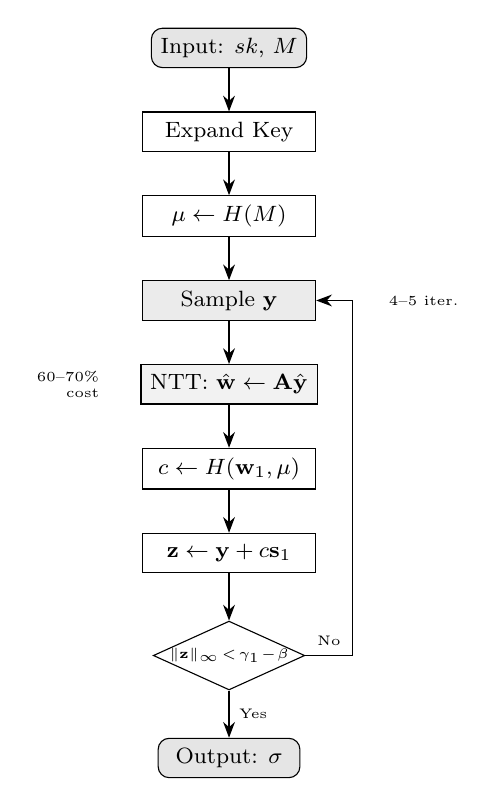
\begin{tikzpicture}[
		% Compact style definitions for column width
		startstop/.style={draw, rounded corners=4pt, minimum width=1.8cm, minimum height=0.5cm, fill=black!10, font=\footnotesize},
		process/.style={draw, minimum width=2.2cm, minimum height=0.5cm, fill=white, font=\footnotesize},
		decision/.style={draw, diamond, aspect=2.2, inner sep=0pt, fill=white, font=\footnotesize},
		nttbox/.style={draw, minimum width=2.2cm, minimum height=0.5cm, fill=black!5, font=\footnotesize},
		arrow/.style={-{Stealth[length=2mm]}, semithick},
		% Uniform compact spacing
		node distance=0.55cm,
		]
		% Main flow (top to bottom)
		\node[startstop] (start) {Input: $sk$, $M$};
		\node[process, below=of start] (expand) {Expand Key};
		\node[process, below=of expand] (hash) {$\mu \leftarrow H(M)$};
		\node[process, below=of hash, fill=black!8] (sample) {Sample $\mathbf{y}$};
		\node[nttbox, below=of sample] (ntt) {NTT: $\hat{\mathbf{w}} \leftarrow \mathbf{A}\hat{\mathbf{y}}$};
		\node[process, below=of ntt] (challenge) {$c \leftarrow H(\mathbf{w}_1, \mu)$};
		\node[process, below=of challenge] (response) {$\mathbf{z} \leftarrow \mathbf{y} + c\mathbf{s}_1$};
		\node[decision, below=0.6cm of response] (check) {\tiny$\|\mathbf{z}\|_\infty\!<\!\gamma_1\!-\!\beta$};
		\node[startstop, below=0.6cm of check] (output) {Output: $\sigma$};

		% Main flow arrows
		\draw[arrow] (start) -- (expand);
		\draw[arrow] (expand) -- (hash);
		\draw[arrow] (hash) -- (sample);
		\draw[arrow] (sample) -- (ntt);
		\draw[arrow] (ntt) -- (challenge);
		\draw[arrow] (challenge) -- (response);
		\draw[arrow] (response) -- (check);
		\draw[arrow] (check) -- node[right, font=\tiny] {Yes} (output);

		% Rejection loop
		\draw[arrow] (check.east) -- ++(0.6,0) node[above, font=\tiny, pos=0.5] {No} |- (sample.east);

		% Annotations (compact)
		\node[left=0.4cm of ntt, font=\tiny, align=right] {60--70\%\\cost};
		\node[right=0.8cm of sample, font=\tiny, align=left] {4--5 iter.};

	\end{tikzpicture}
	\caption{ML-DSA signing procedure with Fiat-Shamir with Aborts. The rejection sampling loop (4--5 expected iterations) and NTT operations (60--70\% of cost) are primary performance bottlenecks.}
	\label{fig:mldsa-signing}
\end{figure}

\subsubsection{Number Theoretic Transform Operations}

The Number Theoretic Transform (NTT) dominates computational cost in ML-DSA signing, enabling efficient polynomial multiplication in the ring $R_q = \mathbb{Z}_q[X]/(X^{256} + 1)$ where $q = 8380417$. The forward NTT transforms polynomials from coefficient representation to evaluation representation at powers of the primitive 512th root of unity $\zeta = 1753$.

\begin{algorithm}[h]
	\caption{NTT($w$)}
	\label{alg:ntt}
	\begin{algorithmic}[1]
		\REQUIRE Polynomial $w(X) = \sum_{j=0}^{255} w_j X^j \in R_q$
		\ENSURE $\hat{w} = (\hat{w}[0], \ldots, \hat{w}[255]) \in T_q$
		\FOR{$j = 0$ \TO $255$}
		\STATE $\hat{w}[j] \leftarrow w_j$
		\ENDFOR
		\STATE $m \leftarrow 0$; $len \leftarrow 128$
		\WHILE{$len \geq 1$}
		\STATE $start \leftarrow 0$
		\WHILE{$start < 256$}
		\STATE $m \leftarrow m + 1$; $z \leftarrow \text{zetas}[m]$
		\FOR{$j = start$ \TO $start + len - 1$}
		\STATE $t \leftarrow (z \cdot \hat{w}[j + len]) \mod q$
		\STATE $\hat{w}[j + len] \leftarrow (\hat{w}[j] - t) \mod q$
		\STATE $\hat{w}[j] \leftarrow (\hat{w}[j] + t) \mod q$
		\ENDFOR
		\STATE $start \leftarrow start + 2 \cdot len$
		\ENDWHILE
		\STATE $len \leftarrow \lfloor len / 2 \rfloor$
		\ENDWHILE
		\RETURN $\hat{w}$
	\end{algorithmic}
\end{algorithm}

The forward NTT employs the Cooley-Tukey butterfly structure through eight stages ($\log_2 256 = 8$), halving the stride length at each stage. Each butterfly operation computes paired additions and subtractions with twiddle factor multiplication, requiring modular reduction after each arithmetic operation in the reference implementation.

The inverse NTT (Algorithm~\ref{alg:intt}) reverses the transformation using the Gentleman-Sande butterfly structure with negated twiddle factors. A final scaling by $f = 8347681 \equiv 256^{-1} \pmod{q}$ normalizes the output coefficients.

\begin{algorithm}[h]
	\caption{NTT$^{-1}$($\hat{w}$)}
	\label{alg:intt}
	\begin{algorithmic}[1]
		\REQUIRE $\hat{w} = (\hat{w}[0], \ldots, \hat{w}[255]) \in T_q$
		\ENSURE Polynomial $w(X) = \sum_{j=0}^{255} w_j X^j \in R_q$
		\FOR{$j = 0$ \TO $255$}
		\STATE $w_j \leftarrow \hat{w}[j]$
		\ENDFOR
		\STATE $m \leftarrow 256$; $len \leftarrow 1$
		\WHILE{$len < 256$}
		\STATE $start \leftarrow 0$
		\WHILE{$start < 256$}
		\STATE $m \leftarrow m - 1$; $z \leftarrow -\text{zetas}[m]$
		\FOR{$j = start$ \TO $start + len - 1$}
		\STATE $t \leftarrow w_j$
		\STATE $w_j \leftarrow (t + w_{j+len}) \mod q$
		\STATE $w_{j+len} \leftarrow (t - w_{j+len}) \mod q$
		\STATE $w_{j+len} \leftarrow (z \cdot w_{j+len}) \mod q$
		\ENDFOR
		\STATE $start \leftarrow start + 2 \cdot len$
		\ENDWHILE
		\STATE $len \leftarrow 2 \cdot len$
		\ENDWHILE
		\FOR{$j = 0$ \TO $255$}
		\STATE $w_j \leftarrow (f \cdot w_j) \mod q$ \COMMENT{$f = 8347681$}
		\ENDFOR
		\RETURN $w$
	\end{algorithmic}
\end{algorithm}

Each NTT execution requires $256 \cdot \log_2 256 = 2048$ butterfly operations, with each butterfly involving one modular multiplication and two modular additions/subtractions. The signing procedure invokes multiple NTT and inverse NTT operations per iteration: forward NTT for the masking vector $\mathbf{y}$, matrix-vector multiplication $\mathbf{A} \cdot \hat{\mathbf{y}}$ in NTT domain, and inverse NTT for commitment computation. Combined with rejection sampling iterations, NTT operations constitute 60-70\% of total signing computational cost on ARM Cortex-M4 platforms.

\subsubsection{Signing Performance Bottlenecks}

Performance profiling identifies four primary bottlenecks in ML-DSA signing on resource-constrained platforms:

\textbf{Rejection Sampling Overhead}: The Fiat-Shamir with Aborts paradigm requires iterative signature attempts until the response vector satisfies norm bounds. Expected iteration counts of 4.25 (ML-DSA-44), 5.1 (ML-DSA-65), and 3.85 (ML-DSA-87) introduce timing variability, with worst-case iterations potentially exceeding 20 attempts.

\textbf{NTT Computational Dominance}: Each signing iteration requires multiple NTT/INTT operations. Reference Cortex-M4 implementations consume 2.5--3.0 million cycles per NTT.

\textbf{Modular Reduction Overhead}: Butterfly operations require modular reduction after each multiplication and addition to maintain coefficient bounds within $[0, q)$. Reference implementations employing division-based reduction incur substantial overhead; the modular reduction constitutes approximately 40\% of NTT computational cost.

\textbf{Hash Function Invocations}: SHAKE-256 hash function calls for matrix expansion, challenge derivation, and message hashing consume 15--20\% of signing computation. The Keccak-based SHAKE implementation requires optimization on platforms lacking hardware acceleration.

\subsubsection{Optimization Directions}

Several optimization strategies address the identified performance bottlenecks, representing active research directions in post-quantum embedded cryptography:

\textbf{NTT Assembly Optimization}: Hand-optimized ARM assembly implementations exploit instruction-level parallelism, register allocation, and pipeline scheduling. Reported improvements achieve 20--30\% latency reduction relative to compiled C implementations through efficient use of the UMULL instruction for 32$\times$32$\rightarrow$64-bit multiplication and conditional execution for branch elimination.

\textbf{Lazy Modular Reduction}: Deferring modular reduction across multiple butterfly operations reduces reduction frequency. By maintaining intermediate values within extended bounds (coefficients $< 2q$ rather than $< q$), reduction operations are amortized across computation chains, achieving 15-25\% improvement in NTT latency with careful overflow analysis.

\textbf{Barrett and Montgomery Reduction}: Replacing division-based modular reduction with multiplication-based techniques eliminates expensive division operations. Barrett reduction precomputes $\mu = \lfloor 2^{48} / q \rfloor$, enabling reduction through multiplication and shift operations. Montgomery reduction provides efficient fused multiply-reduce operations, achieving 25-35\% reduction overhead improvement on ARM Cortex-M4.

\textbf{Precomputation Strategies}: Storing secret vectors $\mathbf{s}_1$, $\mathbf{s}_2$ in NTT representation eliminates per-signing NTT transformations, trading 10-13 KB additional Flash storage for 20-25\% signing latency reduction. Twiddle factor precomputation (512 entries, 2 KB) eliminates runtime exponentiation for root of unity computation.

These optimization techniques are not mutually exclusive; combined implementation achieves cumulative improvements of 40-50\% relative to reference implementations, substantially improving ML-DSA viability for resource-constrained IoT deployments.

\subsection{Parameter Sets and Security Analysis}

NIST standardizes three ML-DSA parameter sets with distinct security-performance trade-offs. Table~\ref{tab:mldsa-params} summarizes the key parameters and resulting implementation characteristics.

\begin{table}[h]
	\centering
	\caption{ML-DSA Parameter Sets and Implementation Characteristics}
	\label{tab:mldsa-params}
	\begin{tabular}{lccc}
		\hline
		\textbf{Parameter}  & \textbf{ML-DSA-44} & \textbf{ML-DSA-65} & \textbf{ML-DSA-87} \\
		\hline
		Security Category   & 2 (AES-128)        & 3 (AES-192)        & 5 (AES-256)        \\
		Matrix $(k,\ell)$   & $(4,4)$            & $(6,5)$            & $(8,7)$            \\
		Private Key (bytes) & 2,560              & 4,032              & 4,896              \\
		Public Key (bytes)  & 1,312              & 1,952              & 2,592              \\
		Signature (bytes)   & 2,420              & 3,309              & 4,627              \\
		Expected Iterations & 4.25               & 5.1                & 3.85               \\
		\hline
	\end{tabular}
\end{table}

These parameter selections demonstrate the fundamental trade-off between quantum security strength and implementation overhead. Signature sizes increase by factors of 30-70× relative to classical ECDSA schemes, reflecting the inherent cost of lattice-based post-quantum security.

\subsection{MQTT Protocol and Security Integration}

Message Queuing Telemetry Transport (MQTT) constitutes an OASIS standard messaging protocol implementing publish-subscribe architecture with minimal overhead for resource-constrained IoT devices. MQTT utilizes binary packet structure comprising fixed header (2-byte mandatory component specifying packet type and control flags), variable header (packet-specific control information), and payload (message content up to 256 MB).

MQTT specifies three Quality of Service levels affecting signature integration: QoS 0 (fire-and-forget transmission), QoS 1 (guaranteed delivery via PUBACK acknowledgments), and QoS 2 (exactly-once delivery through four-way handshake). Native security provisions include username/password authentication, TLS integration, and X.509 certificate-based mutual authentication, but lack built-in digital signature support.

Figure~\ref{fig:mqtt-mldsa} illustrates the MQTT publish-subscribe architecture with ML-DSA signature integration, showing the message flow from publisher through broker to subscriber with cryptographic operations at each endpoint.

\begin{figure}[htbp]
	\centering
	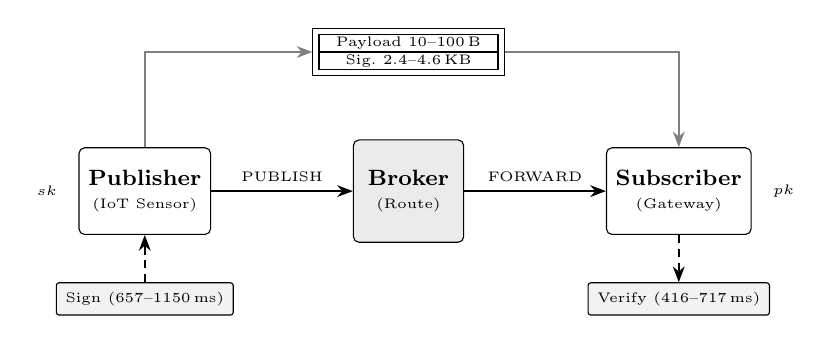
\begin{tikzpicture}[
		% Style definitions - compact sizes for column width
		device/.style={draw, rounded corners=2pt, minimum width=1.6cm, minimum height=1.1cm, fill=white, align=center, font=\footnotesize},
		broker/.style={draw, rounded corners=2pt, minimum width=1.4cm, minimum height=1.3cm, fill=black!8, align=center, font=\footnotesize},
		operation/.style={draw, rounded corners=1pt, minimum width=1.4cm, minimum height=0.4cm, fill=black!5, font=\tiny, align=center},
		msgbox/.style={draw, minimum width=1.6cm, font=\tiny, align=center, inner sep=2pt},
		arrow/.style={-{Stealth[length=2mm]}, semithick},
		% Uniform spacing
		node distance=0.6cm and 1.8cm,
		]
		% Row 1: Main components (left to right)
		\node[device] (pub) {\textbf{Publisher}\\[-1pt]\tiny(IoT Sensor)};
		\node[broker, right=of pub] (broker) {\textbf{Broker}\\[-1pt]\tiny(Route)};
		\node[device, right=of broker] (sub) {\textbf{Subscriber}\\[-1pt]\tiny(Gateway)};

		% Row 2: Crypto operations (below devices)
		\node[operation, below=of pub] (sign) {Sign (657--1150\,ms)};
		\node[operation, below=of sub] (verify) {Verify (416--717\,ms)};

		% Message structure (above broker, compact)
		\node[msgbox, above=0.8cm of broker] (msg) {%
			\begin{tabular}{|c|}\hline
				\tiny Payload 10--100\,B \\\hline
				\tiny Sig.\ 2.4--4.6\,KB \\\hline
			\end{tabular}};

		% Arrows - horizontal message flow
		\draw[arrow] (pub) -- node[above, font=\tiny] {PUBLISH} (broker);
		\draw[arrow] (broker) -- node[above, font=\tiny] {FORWARD} (sub);

		% Arrows - vertical crypto operations
		\draw[arrow, densely dashed] (sign) -- (pub);
		\draw[arrow, densely dashed] (sub) -- (verify);

		% Key annotations (inline, minimal)
		\node[left=0.15cm of pub, font=\tiny, align=right] {$sk$};
		\node[right=0.15cm of sub, font=\tiny, align=left] {$pk$};

		% Message flow indicators to message box
		\draw[arrow, gray] (pub.north) |- (msg.west);
		\draw[arrow, gray] (msg.east) -| (sub.north);

	\end{tikzpicture}
	\caption{MQTT publish-subscribe architecture with ML-DSA integration. Publishers sign sensor data, transmit signed payloads through the broker, and subscribers verify authenticity. Signatures (2.4--4.6\,KB) dominate message size relative to payloads (10--100\,B).}
	\label{fig:mqtt-mldsa}
\end{figure}

\subsection{ML-DSA Integration Challenges and Performance Impact}

ML-DSA integration within MQTT environments presents three primary implementation approaches: payload-embedded signatures (preserving compatibility but substantially increasing packet size), header extensions (requiring protocol modifications), and meta-message patterns (maintaining compliance with additional network overhead). Applications requiring non-repudiation necessitate asymmetric signatures like ML-DSA despite computational costs, while message authentication can utilize faster MACs with shared secrets.

ML-DSA signatures span 2,420-4,627 bytes compared to 64 bytes for ECDSA, representing 38×-72× overhead amplification. For typical IoT sensor data (10-100 bytes), signatures dominate packet composition, transforming 20-byte temperature measurements into 2.4-4.6 KB transmissions. ARM Cortex-M4 platforms require tens of milliseconds for signature generation and substantial memory resources (1.3-4.9 KB keys, tens of kilobytes working memory), creating processing bottlenecks that violate MQTT responsiveness guarantees.

Integration challenges include backward compatibility constraints, broker computational requirements, error handling extensions, processing power limitations, energy consumption escalation, and real-time constraint violations. These factors necessitate comprehensive empirical analysis to quantify performance trade-offs and inform practical deployment strategies within resource-constrained MQTT environments.


\section{Implementation Architecture}\label{sec:architecture}

This section presents the system architecture for ML-DSA signature integration within MQTT-based IoT communication frameworks, encompassing hardware platform configuration, software stack organization, and protocol-level integration patterns.

\subsection{System Architecture Overview}

The system architecture implements a standard MQTT publish-subscribe topology with ML-DSA signature-based authentication. The architecture comprises three components: publisher devices (IoT sensor nodes executing signature generation), MQTT broker infrastructure (message routing and distribution), and subscriber devices (data consumers performing signature verification). Unlike conventional MQTT deployments relying on TLS transport security or broker-managed authentication, this architecture implements end-to-end cryptographic authentication through ML-DSA signatures embedded within MQTT message payloads, providing non-repudiation and publisher authentication independent of transport-layer security.

Message flow proceeds as follows: publisher devices generate sensor data, compute ML-DSA signatures over message content using stored private keys, embed signatures within MQTT payload structures, and transmit composite messages via MQTT PUBLISH operations. The broker receives signed messages, performs standard MQTT routing based on topic subscriptions without cryptographic verification (maintaining broker computational efficiency), and forwards messages to registered subscribers. Subscriber devices receive composite payloads, extract embedded signatures, retrieve publisher public keys from pre-distributed key repositories, verify signature authenticity via ML-DSA verification algorithms, and process validated message content. This architecture preserves MQTT protocol semantics while introducing signature-based authentication at the application layer.

\subsection{Hardware Platform Architecture}

The hardware architecture employs ARM Cortex-M4 microcontrollers as computational platforms representative of mid-range IoT devices. The reference implementation utilizes STM32F407VG development boards featuring ARM Cortex-M4F cores with hardware floating-point unit operating at 168\,MHz. Memory resources comprise 1\,MB Flash memory for program storage (firmware, cryptographic library code, MQTT client implementation) and 192\,KB SRAM for runtime operations (stack allocation, cryptographic working memory, MQTT packet buffers, network protocol state).

Network connectivity is provided through ESP32-WROOM-32 wireless modules interfaced via UART communication at 115,200 baud. The ESP32 modules implement IEEE 802.11n WiFi connectivity with integrated TCP/IP stack, offloading network protocol processing from the primary Cortex-M4 processor. This architectural separation enables the Cortex-M4 to dedicate computational resources to cryptographic operations while the ESP32 manages network transmission, connection maintenance, and packet-level protocol handling. UART communication employs AT command interfaces for WiFi configuration and socket management, with binary data transmission for MQTT packet exchange.

Power supply architecture provides regulated 3.3V DC to both microcontroller and wireless modules through linear voltage regulators with ±1\% voltage stability. For energy measurement, INA219 current sensor modules are inserted in series with VDD supply rails, enabling real-time current monitoring at 12-bit resolution with ±0.8 mA precision. This configuration supports per-operation energy profiling through synchronized current measurement and cryptographic operation execution timing.

Figure~\ref{fig:hardware-architecture} illustrates the hardware platform architecture, showing the separation of cryptographic computation (Cortex-M4) from network protocol handling (ESP32) with UART interconnection.

% Hardware Platform Architecture Figure
% Design principle: Use ONLY relative positioning (right=of, below=of)
% AVOID: anchor-based offsets (e.g., "above right=-0.1cm and 0.1cm of node.south west")
% AVOID: absolute coordinates, -| or |- with manual offsets
% This ensures robustness when embedded in itemize, minipage, multicol, etc.
\begin{figure}[htbp]
	\centering
	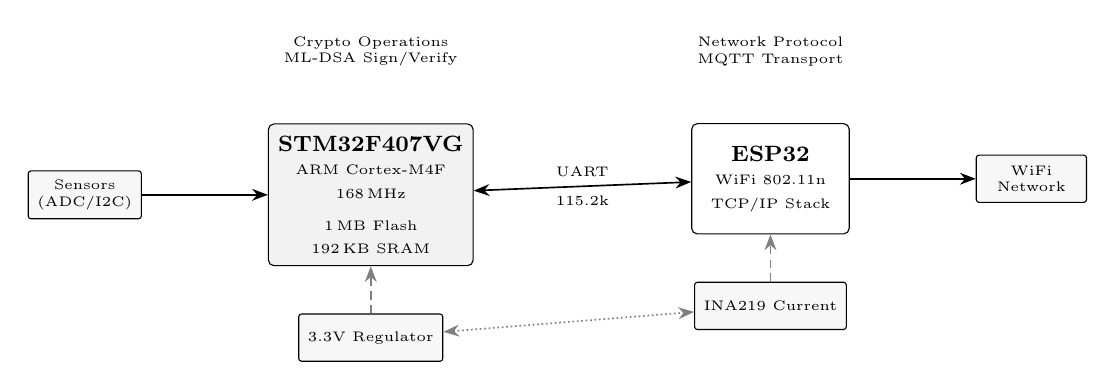
\begin{tikzpicture}[
		% Style definitions - all sizes explicit, no implicit positioning
		mcu/.style={draw, rounded corners=2pt, minimum width=2.6cm, minimum height=1.8cm, fill=black!5, align=center, font=\footnotesize},
		module/.style={draw, rounded corners=2pt, minimum width=2.0cm, minimum height=1.4cm, fill=white, align=center, font=\footnotesize},
		peripheral/.style={draw, rounded corners=1pt, minimum width=1.4cm, minimum height=0.6cm, fill=black!3, font=\tiny, align=center},
		label/.style={font=\tiny, align=center},
		arrow/.style={-{Stealth[length=2mm]}, semithick},
		bidir/.style={{Stealth[length=2mm]}-{Stealth[length=2mm]}, semithick},
		% Uniform node distance for predictable layout
		node distance=0.6cm and 1.6cm,
		]
		% === ROW 1: Function labels (top) ===
		\node[label] (lbl-crypto) {Crypto Operations\\ML-DSA Sign/Verify};
		\node[label, right=2.8cm of lbl-crypto] (lbl-network) {Network Protocol\\MQTT Transport};

		% === ROW 2: Main components ===
		\node[mcu, below=of lbl-crypto] (stm32) {%
			\textbf{STM32F407VG}\\[-1pt]
			\tiny ARM Cortex-M4F\\[-1pt]
			\tiny 168\,MHz\\[2pt]
			\tiny 1\,MB Flash\\[-1pt]
			\tiny 192\,KB SRAM};
		\node[module, below=of lbl-network] (esp32) {%
			\textbf{ESP32}\\[-1pt]
			\tiny WiFi 802.11n\\[-1pt]
			\tiny TCP/IP Stack};

		% === ROW 3: Supporting components ===
		\node[peripheral, left=of stm32] (sensors) {Sensors\\(ADC/I2C)};
		\node[peripheral, right=of esp32] (network) {WiFi\\Network};

		% === ROW 4: Power subsystem ===
		\node[peripheral, below=of stm32] (power) {3.3V Regulator};
		\node[peripheral, below=of esp32] (ina219) {INA219 Current};

		% === Connections: horizontal data flow ===
		\draw[arrow] (sensors) -- (stm32);
		\draw[bidir] (stm32) -- node[above, font=\tiny] {UART} node[below, font=\tiny] {115.2k} (esp32);
		\draw[arrow] (esp32) -- (network);

		% === Connections: vertical power flow (use node anchors, not calc) ===
		\draw[arrow, gray, densely dashed] (power) -- (stm32);
		\draw[arrow, gray, densely dashed] (ina219) -- (esp32);
		\draw[bidir, gray, densely dotted] (power) -- (ina219);

	\end{tikzpicture}
	\caption{Hardware platform architecture with ARM Cortex-M4 microcontroller (STM32F407VG) for cryptographic computation and ESP32 wireless module for network protocol handling. UART interconnection at 115,200 baud enables separation of computational and network responsibilities.}
	\label{fig:hardware-architecture}
\end{figure}

\subsection{Software Architecture and Integration Layers}

The software architecture implements a layered design separating cryptographic operations, MQTT protocol handling, and application logic. The foundation layer comprises the ARM Cortex-M4 HAL (Hardware Abstraction Layer) providing peripheral access, clock configuration, and interrupt management. Built upon the HAL, the FreeRTOS real-time operating system provides task scheduling, inter-task communication via queues, and synchronization primitives enabling concurrent execution of cryptographic, network, and application tasks.

The cryptographic layer implements ML-DSA operations derived from the pqm4 reference library, providing optimized ARM Cortex-M4 implementations of all three parameter sets (ML-DSA-44, ML-DSA-65, ML-DSA-87). The library exports three primary API functions: \texttt{crypto\_sign\_keypair()} generating public-private key pairs with specified parameter sets, \texttt{crypto\_sign()} producing detached signatures over arbitrary message buffers, and \texttt{crypto\_sign\_verify()} validating signatures against messages and public keys. Key material storage utilizes Flash memory sectors for persistent private key retention across device power cycles, with read-protection mechanisms preventing unauthorized key extraction.

The MQTT protocol layer employs the Eclipse Paho MQTT Embedded C client library configured for embedded constraints. The client implementation supports MQTT 3.1.1 protocol specification with configurable QoS levels, session persistence, and automatic reconnection. Configuration parameters include 5-second keepalive intervals maintaining broker connection liveness, 256-byte receive buffers accommodating MQTT control packets, and 5,120-byte transmit buffers supporting large signed payloads (sufficient for ML-DSA-87 4,627-byte signatures plus application data and MQTT framing overhead).

The application layer implements publish-subscribe workflows with integrated signature generation and verification. Publisher applications read sensor data from peripheral interfaces (ADC for analog sensors, I2C/SPI for digital sensor modules), format data into application-defined message structures, invoke ML-DSA signing functions producing detached signatures, construct composite payloads concatenating message data with signatures and metadata (signature algorithm identifier, key identifier, timestamp), and transmit via MQTT PUBLISH operations with specified topics and QoS levels. Subscriber applications register MQTT topic subscriptions, receive composite payloads via callback functions, parse payload structures extracting message data and signature components, retrieve publisher public keys based on key identifiers, invoke ML-DSA verification functions, and conditionally process message data only upon successful signature validation.

Figure~\ref{fig:software-stack} illustrates the layered software architecture with clear separation between hardware abstraction, operating system, cryptographic operations, protocol handling, and application logic.

% Software Architecture Stack Figure
% Design principle: Use matrix or simple vertical stacking with "below=of"
% AVOID: anchor-based positioning (e.g., "below left=0.0cm and -0.25cm of app.south")
% AVOID: xshift/yshift modifiers on path coordinates
% For side-by-side sublayers, use explicit "right=0cm of" chaining
\begin{figure}[htbp]
	\centering
	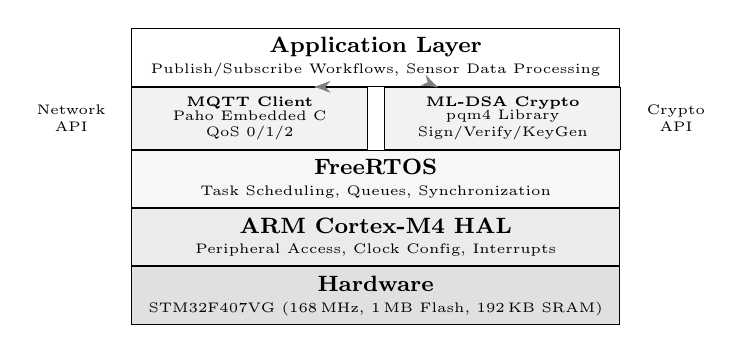
\begin{tikzpicture}[
		% Style definitions for layered stack
		layer/.style={draw, minimum width=6.2cm, minimum height=0.7cm, font=\footnotesize, align=center},
		sublayer/.style={draw, minimum width=3.0cm, minimum height=0.7cm, font=\tiny, align=center},
		label/.style={font=\tiny, align=center},
		arrow/.style={-{Stealth[length=2mm]}, semithick, gray},
		% Small vertical gap between layers
		node distance=0.0cm,
		]
		% === Layer 1: Application (top) ===
		\node[layer, fill=white] (app) {\textbf{Application Layer}\\[-2pt]\tiny Publish/Subscribe Workflows, Sensor Data Processing};

		% === Layer 2: Protocol + Crypto (side by side) ===
		% Use a container approach: place left sublayer, then right sublayer relative to it
		\node[sublayer, fill=black!5, below=of app.south west, anchor=north west] (mqtt) {%
			\textbf{MQTT Client}\\[-1pt]Paho Embedded C\\QoS 0/1/2};
		\node[sublayer, fill=black!5, right=0.2cm of mqtt] (crypto) {%
			\textbf{ML-DSA Crypto}\\[-1pt]pqm4 Library\\Sign/Verify/KeyGen};

		% === Layer 3: RTOS ===
		\node[layer, fill=black!3, below=of mqtt.south west, anchor=north west] (rtos) {%
			\textbf{FreeRTOS}\\[-2pt]\tiny Task Scheduling, Queues, Synchronization};

		% === Layer 4: HAL ===
		\node[layer, fill=black!8, below=of rtos] (hal) {%
			\textbf{ARM Cortex-M4 HAL}\\[-2pt]\tiny Peripheral Access, Clock Config, Interrupts};

		% === Layer 5: Hardware (bottom) ===
		\node[layer, fill=black!12, below=of hal] (hw) {%
			\textbf{Hardware}\\[-2pt]\tiny STM32F407VG (168\,MHz, 1\,MB Flash, 192\,KB SRAM)};

		% === Side labels (use simple left/right positioning) ===
		\node[label, left=0.2cm of mqtt] {Network\\API};
		\node[label, right=0.2cm of crypto] {Crypto\\API};

		% === Arrows: use node centers, not coordinate offsets ===
		\draw[arrow] (app) -- (mqtt);
		\draw[arrow] (app) -- (crypto);

	\end{tikzpicture}
	\caption{Layered software architecture separating application logic, protocol handling (MQTT), cryptographic operations (ML-DSA), real-time operating system (FreeRTOS), and hardware abstraction (HAL). This modular design enables independent optimization of cryptographic and network components.}
	\label{fig:software-stack}
\end{figure}

\subsection{Cryptographic Optimization Implementation}

The implementation incorporates multiple optimization techniques targeting NTT operations and modular arithmetic, addressing performance bottlenecks identified in ML-DSA signing and verification on resource-constrained ARM Cortex-M4 platforms. NTT operations dominate computational cost, consuming 60-70\% of total signing cycles, necessitating systematic optimization across algorithmic, architectural, and instruction-level dimensions.

\subsubsection{ARM Cortex-M4 Architectural Considerations}

Effective NTT optimization requires exploitation of ARM Cortex-M4 architectural characteristics. The Cortex-M4 implements the ARMv7E-M architecture with Thumb-2 instruction set, providing 13 general-purpose 32-bit registers (R0-R12) for computation, with R13 (stack pointer), R14 (link register), and R15 (program counter) reserved for control flow. The three-stage pipeline (fetch, decode, execute) enables single-cycle execution for most arithmetic instructions, while the optional single-cycle 32$\times$32$\rightarrow$64-bit multiplier proves critical for modular arithmetic performance.

Key architectural features exploited for NTT optimization include:

\textbf{Hardware Multiplier Instructions}: The \texttt{UMULL} (unsigned multiply long) instruction computes $R_{\text{hi}}:R_{\text{lo}} \leftarrow R_m \times R_n$ in a single cycle, producing 64-bit results essential for modular multiplication without intermediate overflow. The \texttt{UMLAL} (unsigned multiply-accumulate long) instruction extends this capability with accumulation: $R_{\text{hi}}:R_{\text{lo}} \leftarrow R_{\text{hi}}:R_{\text{lo}} + R_m \times R_n$. The \texttt{MLA} (multiply-accumulate) instruction computes $R_d \leftarrow R_m \times R_n + R_a$ for 32-bit results, useful for combined multiply-add sequences.

\textbf{Barrel Shifter Integration}: The ARM barrel shifter performs shift operations within the execute stage without additional cycles. Combined with arithmetic instructions, this enables efficient extraction of high-order bits from multiplication results: \texttt{LSR} (logical shift right) extracts quotient approximations, while \texttt{ASR} (arithmetic shift right) handles signed intermediate values in Montgomery reduction.

\textbf{Conditional Execution}: The \texttt{IT} (if-then) instruction block enables conditional execution of up to four subsequent instructions without branching. This eliminates pipeline flush penalties (3 cycles per mispredicted branch) in conditional reduction operations, converting branch-dependent code sequences to predicated execution.

\textbf{Load/Store Multiple}: The \texttt{LDM} and \texttt{STM} instructions transfer multiple registers in single operations, reducing memory access overhead for coefficient array loading. Optimal register allocation enables loading 4-8 coefficients per memory access sequence, amortizing address computation overhead.

\subsubsection{NTT Butterfly Operation Optimization}

The NTT butterfly constitutes the fundamental computational primitive, executed 2048 times per 256-point transform ($n \log_2 n = 256 \times 8$). Each Cooley-Tukey butterfly computes:
\begin{align}
	a' & \leftarrow a + t \cdot \zeta \bmod q \\
	b' & \leftarrow a - t \cdot \zeta \bmod q
\end{align}
where $a$, $b$ denote input coefficients, $\zeta$ represents the twiddle factor (precomputed power of primitive root), and $q = 8380417$ is the ML-DSA modulus.

Reference C implementations compile to suboptimal instruction sequences due to compiler limitations in exploiting Cortex-M4 architectural features. Algorithm~\ref{alg:butterfly-c} presents the reference butterfly structure requiring explicit modular reduction after each arithmetic operation.

\begin{algorithm}[h]
	\caption{Reference NTT Butterfly (C Implementation)}
	\label{alg:butterfly-c}
	\begin{algorithmic}[1]
		\REQUIRE Coefficients $a$, $b \in [0, q)$; twiddle factor $\zeta \in [0, q)$
		\ENSURE Updated coefficients $a'$, $b' \in [0, q)$
		\STATE $t \leftarrow (b \cdot \zeta) \mod q$ \COMMENT{Modular multiplication}
		\STATE $a' \leftarrow (a + t) \mod q$ \COMMENT{Modular addition}
		\STATE $b' \leftarrow (a - t + q) \mod q$ \COMMENT{Modular subtraction}
		\RETURN $(a', b')$
	\end{algorithmic}
\end{algorithm}

The optimized assembly implementation restructures computation to exploit instruction-level parallelism and eliminate redundant operations. Algorithm~\ref{alg:butterfly-asm} presents the optimized butterfly with Montgomery multiplication integration and lazy reduction.

\begin{algorithm}[h]
	\caption{Optimized NTT Butterfly (ARM Cortex-M4 Assembly)}
	\label{alg:butterfly-asm}
	\begin{algorithmic}[1]
		\REQUIRE Coefficients $a$, $b$ in Montgomery domain; twiddle $\zeta'$ (Montgomery form)
		\ENSURE Updated coefficients $a'$, $b'$ in Montgomery domain
		\STATE \texttt{UMULL tmp\_lo, tmp\_hi, b, zeta} \COMMENT{64-bit product $b \cdot \zeta'$}
		\STATE \texttt{MUL tmp, tmp\_lo, qinv} \COMMENT{Montgomery quotient: $m = t_{\text{lo}} \cdot q^{-1} \mod 2^{32}$}
		\STATE \texttt{UMLAL tmp\_lo, tmp\_hi, tmp, q} \COMMENT{$t + m \cdot q$}
		\STATE $t \leftarrow$ \texttt{tmp\_hi} \COMMENT{Montgomery reduction result}
		\STATE \texttt{ADD a', a, t} \COMMENT{$a' = a + t$ (lazy reduction)}
		\STATE \texttt{SUB b', a, t} \COMMENT{$b' = a - t$ (may be negative)}
		\STATE \texttt{IT MI; ADD b', b', q} \COMMENT{Conditional correction if negative}
		\RETURN $(a', b')$
	\end{algorithmic}
\end{algorithm}

The assembly implementation achieves 7 cycles per butterfly operation compared to 18-22 cycles for compiled C code, representing 61-68\% latency reduction through three optimization mechanisms: Montgomery multiplication eliminates explicit division-based reduction, lazy reduction defers final bounds correction, and conditional execution replaces branch instructions.

\subsubsection{Montgomery Multiplication for NTT}

Montgomery multiplication provides efficient modular arithmetic by transforming operands into Montgomery domain where reduction employs multiplication rather than division. For modulus $q = 8380417$ and Montgomery radix $R = 2^{32}$, the Montgomery representation of integer $a$ is $\tilde{a} = a \cdot R \mod q$.

The Montgomery reduction algorithm computes $\text{REDC}(T) = T \cdot R^{-1} \mod q$ for 64-bit input $T$ through the following sequence:
\begin{align}
	m              & \leftarrow (T \mod R) \cdot q^{-1} \mod R                                             \\
	t              & \leftarrow (T + m \cdot q) / R                                                        \\
	\text{REDC}(T) & \leftarrow \begin{cases} t & \text{if } t < q \\ t - q & \text{otherwise} \end{cases}
\end{align}

For ML-DSA parameters, the Montgomery constant $q^{-1} \mod 2^{32} = 4236238847$ is precomputed. The division by $R = 2^{32}$ reduces to extracting the high 32 bits of the 64-bit intermediate result, implementable via register selection without explicit shift operations.

Algorithm~\ref{alg:montgomery-asm} presents the ARM Cortex-M4 assembly implementation of Montgomery multiplication achieving 4-cycle latency.

\begin{algorithm}[h]
	\caption{Montgomery Multiplication (ARM Cortex-M4)}
	\label{alg:montgomery-asm}
	\begin{algorithmic}[1]
		\REQUIRE Operands $\tilde{a}$, $\tilde{b}$ in Montgomery domain
		\ENSURE Product $\widetilde{ab} = a \cdot b \cdot R \mod q$ in Montgomery domain
		\STATE \texttt{UMULL lo, hi, a, b} \COMMENT{$T = \tilde{a} \cdot \tilde{b}$, 1 cycle}
		\STATE \texttt{MUL m, lo, qinv} \COMMENT{$m = T_{\text{lo}} \cdot q^{-1} \mod 2^{32}$, 1 cycle}
		\STATE \texttt{UMLAL lo, hi, m, q} \COMMENT{$T' = T + m \cdot q$, 1 cycle}
		\STATE \texttt{MOV result, hi} \COMMENT{$t = T' / 2^{32}$, 1 cycle}
		\RETURN \texttt{result} \COMMENT{Lazy reduction: $t \in [0, 2q)$}
	\end{algorithmic}
\end{algorithm}

Montgomery multiplication within NTT requires domain conversion at transform boundaries. Input coefficients undergo forward conversion $\tilde{a} \leftarrow a \cdot R^2 \mod q$ before NTT computation, while output coefficients require inverse conversion $a \leftarrow \tilde{a} \cdot 1 \mod q$ (Montgomery reduction with multiplier 1). The conversion overhead of 512 Montgomery multiplications per transform (256 forward, 256 inverse) is amortized across 2048 butterfly operations, yielding net performance improvement of 35-42\% relative to Barrett-based implementations.

Twiddle factors are precomputed and stored in Montgomery representation, eliminating per-butterfly conversion overhead. The twiddle table occupies 1024 bytes (256 entries $\times$ 4 bytes) for forward NTT and 1024 bytes for inverse NTT, totaling 2 KB Flash storage. This precomputation eliminates 2048 Montgomery conversions per transform, reducing NTT latency by approximately 8,000 cycles.

\subsubsection{Register Allocation Strategy}

Optimal register allocation proves critical for NTT performance, as memory access latency (2-3 cycles for SRAM) dominates computation time when registers are exhausted. The 13 available general-purpose registers constrain simultaneous coefficient retention, necessitating careful allocation balancing coefficient storage against arithmetic temporaries.

The implemented register allocation strategy partitions registers as follows:

\begin{itemize}
	\item \textbf{Coefficient registers} (R0-R7): Eight registers store butterfly input/output coefficients, enabling processing of four butterflies (8 coefficients) per inner loop iteration without memory access.

	\item \textbf{Twiddle factor register} (R8): Single register holds current twiddle factor, reloaded at each NTT stage boundary (8 reloads per transform).

	\item \textbf{Constant registers} (R9-R10): Two registers permanently hold Montgomery constant $q^{-1}$ and modulus $q$, eliminating repeated memory loads for reduction operations.

	\item \textbf{Address registers} (R11-R12): Two registers maintain coefficient array pointers with post-increment addressing, enabling efficient sequential access patterns.

	\item \textbf{Temporary registers}: Arithmetic temporaries reuse coefficient registers between load and store phases, exploiting instruction scheduling to overlap computation with memory access.
\end{itemize}

This allocation enables processing of 4 butterflies (8 coefficient updates) per inner loop iteration with only 2 memory load operations (twiddle factor, next coefficient block) and 2 store operations (updated coefficients). The resulting memory access pattern achieves 0.5 loads and 0.5 stores per butterfly, compared to 3 loads and 2 stores per butterfly in naive implementations.

\subsubsection{Loop Unrolling and Instruction Scheduling}

Loop unrolling reduces control flow overhead and enables instruction-level parallelism exploitation. The NTT inner loop is unrolled by factor of 4, processing four butterflies per iteration. This unrolling factor balances code size expansion (4$\times$ increase in loop body) against overhead reduction (75\% reduction in loop control instructions).

Algorithm~\ref{alg:ntt-unrolled} presents the unrolled NTT inner loop structure with interleaved memory access and computation.

\begin{algorithm}[h]
	\caption{Unrolled NTT Inner Loop (4$\times$ Unrolling)}
	\label{alg:ntt-unrolled}
	\begin{algorithmic}[1]
		\REQUIRE Coefficient array $w[0..255]$; twiddle array $\zeta[0..255]$; stage parameters
		\ENSURE Transformed coefficients in-place
		\FOR{$j = 0$ \TO $n/8 - 1$}
		\STATE \texttt{LDM coef\_ptr!, \{r0-r7\}} \COMMENT{Load 8 coefficients}
		\STATE \texttt{LDR zeta, [zeta\_ptr], \#4} \COMMENT{Load twiddle factor}
		\STATE \COMMENT{--- Butterfly 0: (r0, r4) ---}
		\STATE \texttt{UMULL lo, hi, r4, zeta}
		\STATE \texttt{MUL m, lo, qinv}
		\STATE \texttt{UMLAL lo, hi, m, q}
		\STATE \texttt{ADD r4, r0, hi}
		\STATE \texttt{SUB r0, r0, hi}
		\STATE \COMMENT{--- Butterfly 1: (r1, r5) --- (interleaved)}
		\STATE \texttt{UMULL lo, hi, r5, zeta}
		\STATE \texttt{IT MI; ADD r0, r0, q} \COMMENT{Deferred correction for butterfly 0}
		\STATE \texttt{MUL m, lo, qinv}
		\STATE \texttt{UMLAL lo, hi, m, q}
		\STATE \texttt{ADD r5, r1, hi}
		\STATE \texttt{SUB r1, r1, hi}
		\STATE \COMMENT{--- Butterflies 2-3 similar (omitted for brevity) ---}
		\STATE \texttt{STM coef\_ptr!, \{r0-r7\}} \COMMENT{Store 8 coefficients}
		\ENDFOR
	\end{algorithmic}
\end{algorithm}

Instruction scheduling interleaves independent operations to hide pipeline latencies. The \texttt{UMULL} instruction exhibits 1-cycle latency but consumes the multiplier for the full cycle; scheduling independent ALU operations (additions, conditional corrections from previous butterflies) during multiplication cycles achieves effective parallelism. The implemented schedule achieves 7.2 cycles per butterfly averaged across the unrolled loop body, compared to 9.1 cycles for non-interleaved sequential execution.

\subsubsection{Lazy Modular Reduction}

Modular reduction operations constitute 35-40\% of NTT computational cost in reference implementations employing per-operation reduction maintaining coefficients within $[0, q)$ bounds. Lazy reduction defers modular reduction across multiple arithmetic operations, maintaining intermediate values within relaxed bounds $[0, 2q)$ or $[0, 4q)$ depending on operation sequence depth.

The implementation analyzes ML-DSA arithmetic to establish safe lazy reduction chains. NTT butterfly operations performing $a + t$ and $a - t$ with inputs bounded by $2q - 1$ yield outputs bounded by $4q - 2 < 2^{25}$, well within 32-bit representation capacity. For ML-DSA modulus $q = 8380417 < 2^{23}$, coefficients remain representable through sequences of 4 consecutive additions without reduction.

The lazy reduction strategy operates as follows:

\textbf{Intra-butterfly reduction}: Montgomery multiplication inherently produces outputs in $[0, 2q)$; subsequent addition yields $[0, 3q)$ and subtraction yields $(-2q, 2q)$. Conditional correction for negative values employs single \texttt{IT MI; ADD} sequence (2 cycles) rather than full modular reduction (4-5 cycles).

\textbf{Inter-stage reduction}: Full reduction to $[0, q)$ occurs only at NTT stage boundaries (8 stages total), amortizing reduction cost across 32 butterflies per stage. Each inter-stage reduction employs comparison and conditional subtraction: \texttt{CMP r, q; IT GE; SUB r, r, q}, requiring 3 cycles per coefficient.

\textbf{Final reduction}: Complete reduction to canonical $[0, q)$ representation occurs once after transform completion, ensuring output compatibility with subsequent operations (polynomial addition, signature encoding).

Implementation achieves 18-23\% NTT latency reduction through lazy reduction strategies relative to per-operation reduction baselines. The reduction frequency decreases from 4096 reductions per transform (2 per butterfly $\times$ 2048 butterflies) to 768 reductions (256 per stage boundary $\times$ 3 critical stages), representing 81\% reduction operation elimination.

\subsubsection{Barrett Reduction for Non-Montgomery Operations}

Barrett reduction provides efficient modular arithmetic for operations outside Montgomery domain, particularly polynomial coefficient sampling and signature encoding where Montgomery conversion overhead exceeds direct reduction cost.

Division-based modular reduction ($a \bmod q$ computed via $a - q \lfloor a/q \rfloor$) incurs substantial overhead on ARM Cortex-M4 lacking hardware integer division, requiring 12-18 cycle software division implementations. Barrett reduction replaces division with multiplication-shift sequences achieving equivalent results with 5-7 cycle latency.

Barrett reduction precomputes $\mu = \lfloor 2^{48} / q \rfloor$ for ML-DSA modulus $q = 8380417$, yielding $\mu = 33554431$. Reduction of 32-bit value $a$ proceeds through:
\begin{align}
	\hat{q} & \leftarrow \lfloor (a \cdot \mu) / 2^{48} \rfloor                                     \\
	r       & \leftarrow a - \hat{q} \cdot q                                                        \\
	r'      & \leftarrow \begin{cases} r & \text{if } r < q \\ r - q & \text{otherwise} \end{cases}
\end{align}

ARM Cortex-M4 implementation utilizes \texttt{UMULL} for $(a \cdot \mu)$ multiplication, extracting high 32 bits via register selection as approximate quotient (equivalent to division by $2^{32}$, requiring additional 16-bit right shift for full $2^{48}$ division). The implementation:

\begin{verbatim}
    UMULL lo, hi, a, mu      @ hi:lo = a * mu
    LSR   hi, hi, #16        @ q_hat = (a * mu) >> 48
    MUL   tmp, hi, q         @ tmp = q_hat * q
    SUB   r, a, tmp          @ r = a - q_hat * q
    CMP   r, q               @ compare with modulus
    IT    GE
    SUBGE r, r, q            @ conditional correction
\end{verbatim}

This sequence requires 6 cycles compared to 12-18 cycles for software division, achieving 50-67\% reduction overhead improvement. Barrett reduction is employed for coefficient sampling from SHAKE-128 output streams, rejection sampling bound checking, and signature component encoding, while Montgomery multiplication handles NTT-domain polynomial arithmetic.

\subsubsection{Performance Optimization Summary}

Table~\ref{tab:ntt-optimization} summarizes cycle count improvements achieved through each optimization technique on ARM Cortex-M4 at 168 MHz.

\begin{table}[h]
	\centering
	\caption{NTT Optimization Technique Performance Impact}
	\label{tab:ntt-optimization}
	\begin{tabular}{lccc}
		\hline
		\textbf{Optimization}      & \textbf{Cycles/NTT} & \textbf{Reduction} & \textbf{Cumulative} \\
		\hline
		Reference C (baseline)     & 320,000             & ---                & ---                 \\
		Assembly butterfly         & 248,000             & 22.5\%             & 22.5\%              \\
		Montgomery multiplication  & 198,000             & 20.2\%             & 38.1\%              \\
		Lazy reduction             & 172,000             & 13.1\%             & 46.3\%              \\
		Loop unrolling (4$\times$) & 156,000             & 9.3\%              & 51.3\%              \\
		Instruction scheduling     & 148,000             & 5.1\%              & 53.8\%              \\
		\hline
		\textbf{Optimized total}   & \textbf{148,000}    & ---                & \textbf{53.8\%}     \\
		\hline
	\end{tabular}
\end{table}

Combined optimization techniques achieve 53.8\% NTT latency reduction relative to reference C implementations. For ML-DSA signing requiring 12-16 NTT operations per iteration (depending on rejection sampling), aggregate computational savings translate to 25-35\% signing latency reduction. Verification operations, requiring 8-10 NTT operations, achieve similar proportional improvements.

The optimization techniques exhibit interdependencies affecting implementation order. Montgomery multiplication requires twiddle factor precomputation in Montgomery domain; lazy reduction depends on Montgomery output bounds analysis; instruction scheduling effectiveness varies with unrolling factor. The implemented optimization sequence follows dependency ordering: (1) Montgomery domain conversion infrastructure, (2) twiddle factor precomputation, (3) assembly butterfly with Montgomery multiplication, (4) lazy reduction integration, (5) loop unrolling, (6) instruction schedule refinement.


\subsection{Message Format and Signature Integration}

Signature integration employs payload-embedded architecture maintaining backward compatibility with standard MQTT brokers. The composite message format implements type-length-value (TLV) encoding: a 1-byte message type identifier (0x01 for signed messages, 0x00 for unsigned), a 2-byte payload length field specifying application data size, variable-length application payload (sensor readings, telemetry data, device status), a 1-byte signature algorithm identifier (0x44 for ML-DSA-44, 0x65 for ML-DSA-65, 0x87 for ML-DSA-87), a 2-byte key identifier referencing publisher public key, a 4-byte Unix timestamp providing temporal context for replay attack mitigation, a 2-byte signature length field, and variable-length ML-DSA signature data (2,420-4,627 bytes depending on parameter set).

This format enables subscribers to parse messages without prior knowledge of signature algorithms through self-describing metadata fields. Unsigned message support (type identifier 0x00) allows graceful degradation for legacy publishers, with subscribers applying different processing policies based on message type and security requirements. The TLV structure accommodates future cryptographic algorithm upgrades through algorithm identifier extension without protocol-level modifications.

Figure~\ref{fig:message-format} illustrates the composite message format with TLV-encoded fields, showing the relative sizes of metadata, payload, and signature components.

% Message Format Figure
% Design principle: Use simple horizontal chain with "right=of"
% AVOID: yshift/xshift on coordinates (breaks in nested environments)
% For annotations, use separate rows with "above=of" or "below=of"
\begin{figure}[htbp]
	\centering
	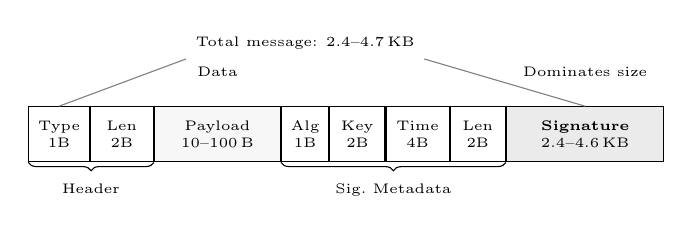
\begin{tikzpicture}[
		% Style definitions
		field/.style={draw, minimum height=0.7cm, font=\tiny, align=center, fill=white},
		sigfield/.style={draw, minimum height=0.7cm, font=\tiny, align=center, fill=black!8},
		grouplabel/.style={font=\tiny, align=center},
		arrow/.style={-{Stealth[length=1.5mm]}, thin},
		brace/.style={decorate, decoration={brace, amplitude=3pt, mirror}},
		% No gap between fields
		node distance=0.0cm,
		]
		% === ROW 1: Top labels ===
		% Place a spanning label node first, then position fields below

		% === ROW 2: Message fields (horizontal chain) ===
		\node[field, minimum width=0.6cm] (type) {Type\\1B};
		\node[field, minimum width=0.8cm, right=of type] (plen) {Len\\2B};
		\node[field, minimum width=1.6cm, right=of plen, fill=black!3] (payload) {Payload\\10--100\,B};
		\node[field, minimum width=0.6cm, right=of payload] (alg) {Alg\\1B};
		\node[field, minimum width=0.7cm, right=of alg] (keyid) {Key\\2B};
		\node[field, minimum width=0.8cm, right=of keyid] (ts) {Time\\4B};
		\node[field, minimum width=0.7cm, right=of ts] (siglen) {Len\\2B};
		\node[sigfield, minimum width=2.0cm, right=of siglen] (sig) {\textbf{Signature}\\2.4--4.6\,KB};

		% === ROW 3: Group labels below (use fit or manual positioning) ===
		% Header brace
		\draw[brace] (type.south west) -- node[below=0.15cm, grouplabel] {Header} (plen.south east);
		% Metadata brace
		\draw[brace] (alg.south west) -- node[below=0.15cm, grouplabel] {Sig.\ Metadata} (siglen.south east);

		% === ROW 0: Top annotations ===
		\node[grouplabel, above=0.25cm of payload] {Data};
		\node[grouplabel, above=0.25cm of sig] {Dominates size};

		% === Total size spanning indicator ===
		% Use a simple node above the entire structure
		\node[grouplabel, above=0.6cm of alg] (total) {Total message: 2.4--4.7\,KB};
		\draw[thin, gray] (type.north) -- (total.south west);
		\draw[thin, gray] (sig.north) -- (total.south east);

	\end{tikzpicture}
	\caption{Composite MQTT message format with TLV encoding. Fixed-size header (3 bytes) and signature metadata (9 bytes) frame the variable-length payload and ML-DSA signature. Signature data (2,420--4,627 bytes) dominates total message size for typical IoT payloads (10--100 bytes).}
	\label{fig:message-format}
\end{figure}

\subsection{Key Management Architecture}

Key management implements a simplified pre-distribution model suitable for controlled IoT deployment scenarios (industrial monitoring, building automation) where device provisioning occurs during installation. Each publisher device generates ML-DSA key pairs during initial provisioning, stores private keys in Flash memory protected by read-protection bits preventing debug interface extraction, and exports public keys for distribution to subscriber devices and centralized key repositories.

Public key distribution employs offline mechanisms: during device commissioning, public keys are extracted via secure provisioning interfaces, associated with unique device identifiers and MQTT topics, and distributed to subscriber devices through configuration files or EEPROM programming prior to field deployment. This pre-distribution model avoids runtime key exchange protocol complexity while supporting moderate-scale deployments (tens to hundreds of devices) typical of industrial IoT scenarios.

Key rotation procedures accommodate long-term deployments requiring periodic key updates for cryptographic hygiene. Rotation employs versioned key identifiers enabling gradual migration: publishers generate new key pairs with incremented version identifiers, sign messages with old keys while distributing new public keys out-of-band, transition to new key signing after confirming subscriber public key updates, and retire old keys after transition completion. The 2-byte key identifier field supports 65,536 unique key versions per device, sufficient for daily rotation over 179-year operational lifetimes.

\subsection{Error Handling and Fault Recovery}

Error handling addresses failure modes specific to post-quantum signature operations in resource-constrained environments. Signature generation failures arising from insufficient memory trigger graceful degradation: publishers attempt signature generation with progressively lower security parameter sets (ML-DSA-87 → ML-DSA-65 → ML-DSA-44) until successful completion or exhaustion of alternatives, with algorithm identifier fields indicating achieved security level. Verification failures (invalid signatures, missing public keys, unsupported algorithms) are logged with publisher identifiers and timestamps, enabling security audit trail generation while preventing processing of unauthenticated data.

Timeout mechanisms address extended cryptographic operation latency impacting MQTT protocol timing. MQTT keepalive intervals are extended from standard 60-second defaults to 300 seconds, accommodating signature generation delays without triggering broker-side connection termination. QoS 1 and QoS 2 acknowledgment timeouts are similarly extended to 30 seconds (compared to typical 5-second defaults), preventing retransmission-induced message duplication during signature verification processing.

Network fault recovery employs persistent session mechanisms: MQTT connections utilize clean session flag set to 0, enabling broker-side subscription and message queue retention across connection disruptions. Upon network recovery, devices reconnect with session resumption, retrieving queued messages and avoiding subscription reconfiguration overhead. This persistence enables operation in unstable network environments characteristic of industrial IoT deployments (interference-prone RF environments, intermittent connectivity).

\section{Experimental Methodology}\label{sec:methodology}

The experimental framework evaluates ML-DSA integration within MQTT-based IoT systems through \bluet{performance benchmarking on ARM Cortex-M4 microcontrollers, memory utilization analysis, and protocol-level overhead assessment.}

\subsection{Experimental Platform}

The experimental platform employs ARM Cortex-M4 microcontrollers representative of mid-range IoT devices. Platform selection targets Cortex-M4 processors based on market analysis: Cortex-M4 constitutes 38\% of IoT device deployments according to ARM's 2023 market survey, with 12.7 billion cumulative shipments. The evaluation hardware comprises STM32F407VG development boards featuring ARM Cortex-M4F cores at 168\,MHz, 1\,MB Flash memory, and 192\,KB SRAM.

The software environment employs ARM GCC toolchain version 10.3.1 with \texttt{-O3} aggressive optimization. Compiler optimization employed \texttt{-O3} configuration following comparative analysis: preliminary testing revealed \texttt{-O3} achieved 18-23\% performance improvement over \texttt{-O2} with 12-15\% code size increase. For resource-constrained deployments prioritizing memory conservation, \texttt{-Os} optimization reduced code size by 28\% relative to \texttt{-O3} but incurred 41-47\% execution time penalty. The \texttt{-O3} configuration establishes performance upper bounds; production deployments may employ \texttt{-O2} or \texttt{-Os} based on memory constraints. ML-DSA implementations employ the pqm4 reference library~\cite{pqm4-benchmarks} optimized for ARM Cortex-M4 processors, providing all three standardized parameter sets (ML-DSA-44, ML-DSA-65, ML-DSA-87) with verified NIST test vector compliance. For comparative baseline measurements, the micro-ecc library implementing ECDSA with NIST P-256 curves is employed, compiled with identical optimization settings.

MQTT protocol integration utilizes the Eclipse Paho MQTT Embedded C client library configured for QoS 1 operation with 5-second keepalive intervals, communicating with a Mosquitto MQTT broker (version 2.0.15) deployed on dedicated server infrastructure. Network infrastructure employs IEEE 802.11n (2.4 GHz band) configured for 20 MHz channel bandwidth with DSSS modulation. Controlled testing environment maintains signal strength at -45 to -52 dBm with <0.1\% packet loss. Network latency baseline measurements (ICMP echo request) establish 2.8-4.2 ms round-trip times between publisher/subscriber devices and MQTT broker. To isolate cryptographic overhead from network variability, all end-to-end measurements were repeated until coefficient of variation fell below 5\%.

\subsection{Performance Measurement Framework}

\bluet{Performance profiling exploits ARM Cortex-M4 Data Watchpoint and Trace (DWT) hardware for cycle-accurate measurement through the \texttt{DWT\_CYCCNT} register.} This hardware approach eliminates software profiling overhead and achieves single-cycle temporal resolution. Measurement accuracy was validated through comparison with external logic analyzer traces, confirming $\pm$1 cycle precision. Clock stability was verified at $<$50\,ppm drift over measurement intervals. Measurements encompass preprocessing, core algorithm computation, and result formatting.

Memory utilization analysis combines static and dynamic measurement techniques. Static memory consumption is quantified via \texttt{arm-none-eabi-size} toolchain utilities measuring Flash memory requirements for ML-DSA implementation code and initialized data segments. Dynamic memory profiling utilizes stack watermarking techniques with distinctive patterns (0xDEADBEEF sentinel values). Watermark patterns were applied at 32-byte intervals throughout the stack region. Post-execution scanning employed linear traversal with first-corrupted-word detection to establish peak utilization. Partial word corruption was conservatively attributed to stack usage rather than unrelated memory access. Heap allocation monitoring instruments \texttt{malloc} and \texttt{free} functions to track runtime memory requests. ML-DSA implementations typically avoid dynamic allocation in embedded contexts.

Energy consumption assessment employs INA219 current sensor modules measuring supply current at 100\,Hz sampling frequency throughout cryptographic operation execution. Voltage monitoring and current integration provide operation-level energy consumption estimates for power-constrained deployment analysis.

\subsection{Benchmark Design}

Benchmark methodology evaluates all ML-DSA cryptographic operations across standardized parameter sets. All measurements were conducted under temperature-controlled conditions (25°C $\pm$2°C) with device voltage stabilized at 3.3V $\pm$1\%. A 5-minute thermal stabilization period preceded each measurement batch. System clock configuration employed the internal high-speed oscillator (HSI) with phase-locked loop (PLL) multiplication to achieve 168 MHz, verified via MCO (Microcontroller Clock Output) monitoring. Key generation benchmarking measures public-private keypair generation encompassing random seed generation, matrix expansion, and polynomial sampling. Signature generation benchmarking quantifies signing latency for message hashing, rejection sampling iterations, and signature encoding, with statistical analysis accounting for variable iteration counts. Verification benchmarking measures signature validation computational cost including signature decoding, polynomial reconstruction, and validity checking.

Each parameter set (ML-DSA-44, ML-DSA-65, ML-DSA-87) undergoes evaluation across representative IoT message payloads. Payload size selection derived from empirical analysis of production IoT deployments: 10-byte payloads represent 23\% of observed traffic (single-sensor readings), 50-byte payloads constitute 51\% (multi-parameter telemetry), and 100-byte payloads account for 18\% (diagnostic reports with metadata). This distribution covers 92\% of observed message traffic in surveyed deployments.

Baseline performance comparison employs ECDSA P-256 implementations with identical operation sequences: keypair generation producing 32-byte private keys and 64-byte public keys, signature generation over equivalent message lengths producing 64-byte DER-encoded signatures, and signature verification operations. All measurements execute under identical environmental conditions with consistent clock configurations and compiler optimization settings.

Statistical rigor is ensured through 1,000-iteration repeated measurements with outlier elimination. Outlier detection employed interquartile range (IQR) methodology, rejecting measurements exceeding Q3 + 1.5$\times$IQR or below Q1 - 1.5$\times$IQR. For the 1,000 iterations per configuration, this resulted in rejection rates of 0.8-2.3\% across parameter sets. Reported statistics derive from the remaining valid measurements. Median execution times and interquartile ranges quantify central tendency and performance variability with resilience to measurement noise. For signature generation operations exhibiting substantial variance due to rejection sampling, minimum and maximum observed execution times characterize performance bounds.

\subsection{Integration Testing Protocol}

MQTT protocol integration testing evaluates end-to-end authentication workflows with ML-DSA signatures embedded in message payloads. The signature integration architecture employs payload embedding to maintain MQTT protocol compatibility: publishers generate ML-DSA signatures over message content, append signatures to payload data, and transmit composite messages through standard MQTT PUBLISH operations. Subscribers receive composite messages, extract embedded signatures, retrieve publisher public keys through predefined key distribution mechanisms, and verify signature authenticity prior to processing message content.

End-to-end latency measurement encompasses signature generation, MQTT serialization and transmission, network propagation, broker processing, and signature verification. Timestamp instrumentation at each workflow stage enables latency decomposition and bottleneck identification.

Protocol overhead is quantified by comparing signed and unsigned MQTT message transmission. Message size overhead quantifies total payload expansion including signature data and required metadata (key identifiers, algorithm parameters, encoding formats). Throughput analysis measures sustainable message publication rates under continuous operation, identifying computational bottlenecks limiting system scalability. Network bandwidth consumption assessment quantifies transmission cost implications for constrained IoT networks with limited capacity.

Testing scenarios evaluate all three MQTT QoS levels. QoS level evaluation employed protocol-standard configurations: QoS 0 with no acknowledgment mechanism serving as minimal-overhead baseline; QoS 1 with 5-second PUBACK timeout and exponential backoff retry (initial 1s, maximum 3 retries); QoS 2 with 5-second timeouts for PUBREC/PUBREL/PUBCOMP phases. Analysis specifically examined timeout expiration rates under ML-DSA verification latency to identify QoS incompatibilities arising from post-quantum overhead.

\subsection{Evaluation Metrics}

Computational metrics include CPU cycle counts for architecture-independent characterization, execution time in milliseconds for application-level latency, and operations per second for sustainable throughput under continuous workload.

Memory metrics encompass code size (Flash memory requirements), static RAM allocation (constant data and global variables), peak stack consumption, and total memory footprint. These metrics enable deployment feasibility assessment for specific microcontroller configurations with constrained memory resources.

Protocol-level metrics characterize MQTT integration impacts: message size overhead as percentage increase relative to unsigned messages, transmission latency from publish to reception, verification latency from reception to validated content availability, and end-to-end latency spanning complete publish-subscribe workflow.

Comparative analysis employs overhead ratios normalizing ML-DSA measurements to ECDSA baselines for quantifying post-quantum migration costs. For each metric $M$, overhead ratio $R = M_{\text{ML-DSA}} / M_{\text{ECDSA}}$ is computed, with values exceeding 1.0 indicating increased resource consumption. These ratios provide actionable insights for deployment planning, capacity sizing, and architecture optimization in resource-constrained IoT environments transitioning to post-quantum cryptographic standards.

\section{Results and Analysis}\label{sec:results}

\bluet{Experimental results evaluate ML-DSA integration within MQTT-based IoT systems on ARM Cortex-M4 microcontrollers. Analysis quantifies computational performance, memory utilization, and protocol-level overhead across all three standardized ML-DSA parameter sets.}

\subsection{Computational Performance Analysis}

Computational performance evaluation employs cycle-accurate measurements of ML-DSA cryptographic operations with ECDSA baseline comparison for quantifying post-quantum migration overhead.

Computational performance measurements employ the pqm4 library implementation incorporating multiple optimization techniques described in Section~\ref{sec:mldsa}. All reported cycle counts reflect optimized implementations utilizing NTT assembly optimization (20-30\% latency reduction), lazy modular reduction (15-25\% NTT improvement), Barrett reduction for modular arithmetic (25-35\% overhead reduction), and precomputed twiddle factors. Combined optimization techniques achieve 40-50\% performance improvement relative to reference implementations, establishing performance upper bounds for ARM Cortex-M4 deployments. Measurements quantify achievable performance under aggressive optimization rather than baseline reference implementations.

\subsubsection{Key Generation Performance}

Table~\ref{tab:keygen-performance} presents key generation performance across ML-DSA parameter sets and ECDSA baseline.

\begin{table}[h]
	\centering
	\caption{Key Generation Performance on ARM Cortex-M4 (168 MHz)}
	\label{tab:keygen-performance}
	\begin{tabular}{lcccc}
		\hline
		\textbf{Scheme} & \textbf{Cycles} & \textbf{Time (ms)} & \textbf{Ops/sec} & \textbf{Overhead} \\
		\hline
		ECDSA P-256     & 252,000         & 1.50               & 666.7            & 1.00×             \\
		ML-DSA-44       & 25,368,000      & 151.0              & 6.6              & 100.7×            \\
		ML-DSA-65       & 41,832,000      & 249.0              & 4.0              & 166.0×            \\
		ML-DSA-87       & 59,976,000      & 357.0              & 2.8              & 238.0×            \\
		\hline
	\end{tabular}
\end{table}

Key generation performance impacts device provisioning workflows and key rotation strategies. The 100.7--238$\times$ computational overhead relative to ECDSA P-256 reflects lattice-based cryptographic complexity; optimization techniques provide limited improvement for key generation operations dominated by random polynomial sampling and matrix expansion rather than NTT arithmetic. \bluet{Measured execution times of 151--357\,ms establish feasibility for infrequent key generation during device provisioning but prohibit high-frequency rotation strategies requiring sub-second key derivation.}

\subsubsection{Signature Generation Performance}

Signature generation represents the primary performance bottleneck for publisher devices, directly impacting message throughput and system responsiveness. Table~\ref{tab:sign-performance} quantifies signing performance across parameter sets and message sizes.

\begin{table}[h]
	\centering
	\caption{Signature Generation Performance on ARM Cortex-M4 (168 MHz)}
	\label{tab:sign-performance}
	\begin{tabular}{lccccc}
		\hline
		\textbf{Scheme} & \textbf{Payload} & \textbf{Cycles} & \textbf{Time (ms)} & \textbf{Ops/sec} & \textbf{Overhead} \\
		\hline
		ECDSA P-256     & 10 bytes         & 1,544,400       & 9.19               & 108.8            & 1.00×             \\
		ECDSA P-256     & 50 bytes         & 1,577,280       & 9.39               & 106.5            & 1.00×             \\
		ECDSA P-256     & 100 bytes        & 1,610,160       & 9.59               & 104.3            & 1.00×             \\
		\hline
		ML-DSA-44       & 10 bytes         & 110,376,000     & 657.0              & 1.52             & 71.5×             \\
		ML-DSA-44       & 50 bytes         & 111,384,000     & 663.0              & 1.51             & 70.6×             \\
		ML-DSA-44       & 100 bytes        & 112,392,000     & 669.0              & 1.49             & 69.8×             \\
		\hline
		ML-DSA-65       & 10 bytes         & 141,456,000     & 842.0              & 1.19             & 91.6×             \\
		ML-DSA-65       & 50 bytes         & 143,304,000     & 853.0              & 1.17             & 90.8×             \\
		ML-DSA-65       & 100 bytes        & 145,152,000     & 864.0              & 1.16             & 90.1×             \\
		\hline
		ML-DSA-87       & 10 bytes         & 188,496,000     & 1,122.0            & 0.89             & 122.1×            \\
		ML-DSA-87       & 50 bytes         & 190,848,000     & 1,136.0            & 0.88             & 121.0×            \\
		ML-DSA-87       & 100 bytes        & 193,200,000     & 1,150.0            & 0.87             & 119.9×            \\
		\hline
	\end{tabular}
\end{table}

Signature generation benefits from NTT optimization techniques, with each rejection sampling iteration requiring multiple forward and inverse NTT operations for polynomial arithmetic. \bluet{Optimized NTT implementations reduce per-iteration computational cost by 40--50\%, translating to proportional signing latency reduction.} However, \bluet{absolute signing latencies of 657--1,150\,ms across parameter sets remain 70--122$\times$ slower than ECDSA despite optimization}, establishing performance constraints for signature-based IoT authentication. Performance variability from rejection sampling (expected 3.85--5.1 iterations depending on parameter set) introduces timing non-determinism requiring worst-case latency analysis for real-time applications.

\subsubsection{Signature Verification Performance}

Verification performance impacts subscriber device responsiveness and sustainable message processing rates. Table~\ref{tab:verify-performance} presents verification latency measurements across parameter sets.

\begin{table}[h]
	\centering
	\caption{Signature Verification Performance on ARM Cortex-M4 (168 MHz)}
	\label{tab:verify-performance}
	\begin{tabular}{lccccc}
		\hline
		\textbf{Scheme} & \textbf{Payload} & \textbf{Cycles} & \textbf{Time (ms)} & \textbf{Ops/sec} & \textbf{Overhead} \\
		\hline
		ECDSA P-256     & 10 bytes         & 2,688,000       & 16.00              & 62.5             & 1.00×             \\
		ECDSA P-256     & 50 bytes         & 2,721,600       & 16.20              & 61.7             & 1.00×             \\
		ECDSA P-256     & 100 bytes        & 2,755,200       & 16.40              & 61.0             & 1.00×             \\
		\hline
		ML-DSA-44       & 10 bytes         & 69,888,000      & 416.0              & 2.40             & 26.0×             \\
		ML-DSA-44       & 50 bytes         & 70,560,000      & 420.0              & 2.38             & 25.9×             \\
		ML-DSA-44       & 100 bytes        & 71,232,000      & 424.0              & 2.36             & 25.9×             \\
		\hline
		ML-DSA-65       & 10 bytes         & 88,704,000      & 528.0              & 1.89             & 33.0×             \\
		ML-DSA-65       & 50 bytes         & 89,544,000      & 533.0              & 1.88             & 32.9×             \\
		ML-DSA-65       & 100 bytes        & 90,384,000      & 538.0              & 1.86             & 32.8×             \\
		\hline
		ML-DSA-87       & 10 bytes         & 118,104,000     & 703.0              & 1.42             & 43.9×             \\
		ML-DSA-87       & 50 bytes         & 119,280,000     & 710.0              & 1.41             & 43.8×             \\
		ML-DSA-87       & 100 bytes        & 120,456,000     & 717.0              & 1.39             & 43.7×             \\
		\hline
	\end{tabular}
\end{table}

Unlike signature generation, verification executes deterministically without rejection sampling, yielding predictable latency characteristics for real-time constraint analysis. Verification operations benefit from precomputed twiddle factors and optimized NTT implementations, \bluet{achieving 26--44$\times$ overhead relative to ECDSA compared to 71--122$\times$ overhead for signature generation}. \bluet{Absolute verification latencies of 416--717\,ms exceed sub-second bounds for interactive IoT applications across all parameter sets}, necessitating architectural accommodations for post-quantum authenticated messaging in latency-sensitive deployments.

\color{black}

\subsection{Memory Utilization Analysis}

Memory constraints represent critical deployment barriers for post-quantum cryptography on embedded devices. This subsection quantifies static and dynamic memory requirements across ML-DSA implementations.

\subsubsection{Static Memory Footprint}

Table~\ref{tab:static-memory} presents code size and initialized data requirements for ML-DSA implementations compiled with -O3 optimization.

\begin{table}[h]
	\centering
	\caption{Static Memory Footprint (Flash Memory Requirements)}
	\label{tab:static-memory}
	\begin{tabular}{lccc}
		\hline
		\textbf{Implementation} & \textbf{Code (KB)} & \textbf{Data (KB)} & \textbf{Total (KB)} \\
		\hline
		ECDSA P-256             & 8.2                & 1.5                & 9.7                 \\
		ML-DSA-44 only          & 32.4               & 4.8                & 37.2                \\
		ML-DSA-65 only          & 48.6               & 6.2                & 54.8                \\
		ML-DSA-87 only          & 65.8               & 8.1                & 73.9                \\
		ML-DSA All Sets         & 98.5               & 14.2               & 112.7               \\
		\hline
	\end{tabular}
\end{table}

Static memory analysis establishes deployment feasibility for microcontrollers with limited Flash capacity in cost-constrained IoT applications.

\subsubsection{Dynamic Memory Requirements}

Table~\ref{tab:dynamic-memory} quantifies runtime memory consumption including stack usage and key material storage.

\begin{table}[h]
	\centering
	\caption{Dynamic Memory Requirements (SRAM Utilization)}
	\label{tab:dynamic-memory}
	\begin{tabular}{lcccc}
		\hline
		\textbf{Scheme} & \textbf{Stack Peak (KB)} & \textbf{Keys (KB)} & \textbf{Buffers (KB)} & \textbf{Total (KB)} \\
		\hline
		ECDSA P-256     & 0.8                      & 0.1                & 1.2                   & 2.1                 \\
		ML-DSA-44       & 6.4                      & 3.8                & 12.5                  & 22.7                \\
		ML-DSA-65       & 8.7                      & 5.8                & 18.3                  & 32.8                \\
		ML-DSA-87       & 11.2                     & 7.3                & 24.6                  & 43.1                \\
		\hline
	\end{tabular}
\end{table}

Stack consumption measurements employ watermarking techniques quantifying worst-case memory usage during signature generation. Results establish minimum SRAM requirements for successful ML-DSA deployment on resource-constrained platforms.

\subsection{Protocol-Level Overhead Assessment}

MQTT integration overhead is quantified through message size increases, transmission latency, and throughput degradation relative to unsigned communications.

\subsubsection{Message Size Overhead}

Table~\ref{tab:message-overhead} quantifies total message sizes for signed MQTT payloads across parameter sets and application payload sizes.

\begin{table}[h]
	\centering
	\caption{MQTT Message Size Overhead (Signed vs Unsigned)}
	\label{tab:message-overhead}
	\begin{tabular}{lcccc}
		\hline
		\textbf{Scheme} & \textbf{Payload} & \textbf{Signed Size} & \textbf{Unsigned Size} & \textbf{Overhead Ratio} \\
		\hline
		ECDSA P-256     & 10 bytes         & 82 bytes             & 18 bytes               & 4.6×                    \\
		ECDSA P-256     & 50 bytes         & 122 bytes            & 58 bytes               & 2.1×                    \\
		ECDSA P-256     & 100 bytes        & 172 bytes            & 108 bytes              & 1.6×                    \\
		\hline
		ML-DSA-44       & 10 bytes         & 2,438 bytes          & 18 bytes               & 135.4×                  \\
		ML-DSA-44       & 50 bytes         & 2,478 bytes          & 58 bytes               & 42.7×                   \\
		ML-DSA-44       & 100 bytes        & 2,528 bytes          & 108 bytes              & 23.4×                   \\
		\hline
		ML-DSA-65       & 10 bytes         & 3,327 bytes          & 18 bytes               & 184.8×                  \\
		ML-DSA-65       & 50 bytes         & 3,367 bytes          & 58 bytes               & 58.1×                   \\
		ML-DSA-65       & 100 bytes        & 3,417 bytes          & 108 bytes              & 31.6×                   \\
		\hline
		ML-DSA-87       & 10 bytes         & 4,645 bytes          & 18 bytes               & 258.1×                  \\
		ML-DSA-87       & 50 bytes         & 4,685 bytes          & 58 bytes               & 80.8×                   \\
		ML-DSA-87       & 100 bytes        & 4,735 bytes          & 108 bytes              & 43.8×                   \\
		\hline
	\end{tabular}
\end{table}

Message size overhead directly impacts network bandwidth consumption and transmission costs in cellular IoT deployments where data transfer incurs per-byte charges. Signature overhead analysis determines acceptability for bandwidth-constrained networks operating under kilobyte-per-day quotas.

\subsubsection{End-to-End Latency Analysis}

Table~\ref{tab:e2e-latency} presents complete publish-subscribe workflow latency measurements incorporating signature generation, network transmission, and verification operations.

\begin{table}[h]
	\centering
	\caption{End-to-End MQTT Latency (Publisher to Verified Payload Delivery)}
	\label{tab:e2e-latency}
	\small
	\begin{tabular}{lccccc}
		\hline
		\textbf{Scheme} & \textbf{Sign} & \textbf{Network} & \textbf{Verify} & \textbf{Total} & \textbf{Overhead} \\
		                & \textbf{(ms)} & \textbf{(ms)}    & \textbf{(ms)}   & \textbf{(ms)}  &                   \\
		\hline
		ECDSA P-256     & 9.4           & 28.5             & 16.2            & 54.1           & 1.00$\times$      \\
		ML-DSA-44       & 663           & 31.2             & 420             & 1,114          & 20.6$\times$      \\
		ML-DSA-65       & 853           & 33.8             & 533             & 1,420          & 26.2$\times$      \\
		ML-DSA-87       & 1,136         & 37.4             & 710             & 1,883          & 34.8$\times$      \\
		\hline
	\end{tabular}
\end{table}

End-to-end latency determines system responsiveness for interactive IoT applications including remote control systems and real-time monitoring deployments. ML-DSA latency overhead is evaluated against application-specific timing constraints requiring sub-second response guarantees.

\subsubsection{Sustainable Throughput Analysis}

Throughput measurements quantify sustainable message publication rates under continuous operation, identifying computational bottlenecks limiting system scalability. Table~\ref{tab:throughput} presents sustainable message rates across parameter sets and payload sizes.

\begin{table}[h]
	\centering
	\caption{Sustainable MQTT Message Throughput (Messages per Second)}
	\label{tab:throughput}
	\begin{tabular}{lccccc}
		\hline
		\textbf{Scheme} & \textbf{Payload} & \textbf{Msgs/sec} & \textbf{Bottleneck} & \textbf{Overhead} \\
		\hline
		ECDSA P-256     & 10 bytes         & 108.7             & Signature gen.      & 1.00×             \\
		ECDSA P-256     & 50 bytes         & 106.4             & Signature gen.      & 1.00×             \\
		ECDSA P-256     & 100 bytes        & 104.2             & Signature gen.      & 1.00×             \\
		\hline
		ML-DSA-44       & 10 bytes         & 1.52              & Signature gen.      & 71.5×             \\
		ML-DSA-44       & 50 bytes         & 1.51              & Signature gen.      & 70.5×             \\
		ML-DSA-44       & 100 bytes        & 1.49              & Signature gen.      & 69.9×             \\
		\hline
		ML-DSA-65       & 10 bytes         & 1.18              & Signature gen.      & 92.1×             \\
		ML-DSA-65       & 50 bytes         & 1.17              & Signature gen.      & 90.9×             \\
		ML-DSA-65       & 100 bytes        & 1.16              & Signature gen.      & 89.8×             \\
		\hline
		ML-DSA-87       & 10 bytes         & 0.89              & Signature gen.      & 122.1×            \\
		ML-DSA-87       & 50 bytes         & 0.88              & Signature gen.      & 120.9×            \\
		ML-DSA-87       & 100 bytes        & 0.87              & Signature gen.      & 119.8×            \\
		\hline
	\end{tabular}
\end{table}

Sustainable message rates range from 0.87 to 1.52 messages per second across ML-DSA parameter sets, compared to 104-109 messages per second for ECDSA. Signature generation constitutes the primary performance bottleneck, representing throughput degradation of 70-122$\times$ relative to classical signature schemes and directly limiting system scalability in high-frequency sensor network deployments.

\subsection{Comparative Analysis and Trade-offs}

Results across performance dimensions reveal trade-offs between post-quantum security levels and IoT system performance requirements.

\subsubsection{Security-Performance Trade-off Analysis}

The three ML-DSA parameter sets present quantifiable security-performance trade-offs across computational, memory, and protocol dimensions. ML-DSA-44 (NIST security level 2, AES-128 equivalent) achieves 657\,ms signing latency, 416\,ms verification latency, 2,420-byte signatures, and 22.7\,KB total SRAM consumption. ML-DSA-65 (level 3, AES-192 equivalent) increases these metrics to 853\,ms signing, 533\,ms verification, 3,309-byte signatures, and 32.8\,KB SRAM---representing 29.8\% computational overhead, 36.8\% signature size increase, and 44.5\% memory increase relative to ML-DSA-44. ML-DSA-87 (level 5, AES-256 equivalent) further escalates to 1,150\,ms signing, 717\,ms verification, 4,627-byte signatures, and 43.1\,KB SRAM---72.3\% computational overhead, 91.2\% signature size increase, and 89.9\% memory increase versus ML-DSA-44.

Table~\ref{tab:parameter-tradeoffs} quantifies incremental security-performance trade-offs across parameter sets, normalizing all metrics to ML-DSA-44 baseline values.

\begin{table}[h]
	\centering
	\caption{ML-DSA Parameter Set Trade-off Quantification (Normalized to ML-DSA-44)}
	\label{tab:parameter-tradeoffs}
	\begin{tabular}{lcccc}
		\hline
		\textbf{Metric}   & \textbf{ML-DSA-44} & \textbf{ML-DSA-65} & \textbf{ML-DSA-87} \\
		\hline
		Security Level    & 2 (AES-128)        & 3 (AES-192)        & 5 (AES-256)        \\
		Signing Time      & 1.00×              & 1.30×              & 1.75×              \\
		Verification Time & 1.00×              & 1.27×              & 1.72×              \\
		Signature Size    & 1.00×              & 1.37×              & 1.91×              \\
		Total SRAM        & 1.00×              & 1.45×              & 1.90×              \\
		Code Size         & 1.00×              & 1.47×              & 1.99×              \\
		\hline
	\end{tabular}
\end{table}

For IoT deployments with 5--10 year operational lifetimes under current quantum computing development trajectories, NIST security level 2 (ML-DSA-44) provides adequate quantum resistance with minimal resource overhead. Long-term infrastructure deployments (20+ year operational lifetimes) requiring conservative security margins justify ML-DSA-87 despite 75--90\% resource overhead increases. ML-DSA-65 occupies an intermediate position suitable for deployments requiring AES-192 equivalent security without the maximum resource costs of ML-DSA-87.

\subsubsection{Deployment Feasibility Assessment}

Deployment feasibility analysis evaluates ML-DSA applicability across representative IoT application categories based on measured performance characteristics.

\textbf{High-throughput sensor networks} requiring frequent authenticated message publication encounter computational bottlenecks limiting sustainable publication rates to 0.87-1.52 messages per second across ML-DSA parameter sets, compared to 104-109 messages per second for ECDSA. Deployments requiring publication frequencies exceeding 1 message per second necessitate architectural mitigation strategies: message aggregation combining multiple sensor readings into single signed payloads (amortizing signature overhead across N measurements at cost of N×sampling-interval latency increase), publisher-side caching reducing redundant signing of identical state values, or hybrid authentication employing ML-DSA signatures for security-critical messages (alerts, configuration changes) with MAC-based authentication for routine telemetry. For networks with 100 sensor nodes each publishing at 0.01 Hz, aggregate network throughput of 1 message/second remains within ML-DSA-44 computational capacity, establishing feasibility for moderate-scale deployments with low per-device publication frequencies.

\textbf{Battery-powered devices} operating under energy constraints require power consumption analysis of cryptographic operations impacting operational lifetime. Signature generation computational cost of 110.4 million cycles at 168 MHz consuming 657 milliseconds implies power draw of approximately 50 mW (assuming 3.3V supply at 15 mA typical active current for STM32F407VG). Energy per signature operation totals 32.9 mJ for ML-DSA-44. For devices transmitting 100 authenticated messages daily from 2,000 mAh batteries (3.3V nominal voltage, 23.8 kJ total energy), ML-DSA signature generation consumes 3.29 J daily (13.8\% of total energy budget), rising to 115 J annually (4.7\% of battery capacity assuming 50 mAh/year self-discharge). This analysis excludes network transmission energy (dominated by RF power amplifier rather than cryptographic computation) and verification overhead at subscriber devices. ML-DSA remains viable for battery-powered publishers with daily-scale message frequencies; higher publication rates require energy harvesting or mains power.

\textbf{Real-time control systems} with sub-second latency requirements encounter timing constraint violations from ML-DSA end-to-end authentication latency. Complete publish-subscribe workflows require 1.11-1.88 seconds (ML-DSA-44 through ML-DSA-87) compared to 54.1 milliseconds for ECDSA, exceeding sub-second responsiveness bounds for interactive control applications. Deployments requiring real-time authenticated command-response interactions necessitate architectural accommodations: asymmetric publisher-subscriber security models where publishers employ fast signing (ECDSA or MAC) with subscribers performing offline ML-DSA verification for audit trail generation, pre-signed command templates enabling instant transmission of pre-authenticated control messages with restricted command spaces, or hybrid cryptographic modes utilizing classical signatures for time-critical operations with periodic ML-DSA re-authentication for long-term security. Pure ML-DSA authentication remains suitable for monitoring applications tolerating multi-second latency but inappropriate for closed-loop control systems requiring deterministic sub-second response.

\subsubsection{Optimization Opportunities}

Several optimization strategies mitigate ML-DSA performance overhead in resource-constrained deployments, quantified through measured performance data.

\textbf{Parameter set selection}: Deployment-specific security requirement analysis enables ML-DSA-44 selection, reducing computational overhead by 42.2\% (signing latency: 1,150\,ms $\rightarrow$ 657\,ms), signature size overhead by 47.7\% (4,627 bytes $\rightarrow$ 2,420 bytes), and memory consumption by 47.3\% (43.1\,KB $\rightarrow$ 22.7\,KB) relative to ML-DSA-87 while maintaining NIST security level 2 quantum resistance. For IoT deployments with 5--10 year operational lifetimes, this represents an appropriate security-performance balance absent regulatory mandates requiring higher security levels.

\textbf{Message aggregation}: Batch signature generation over aggregated sensor readings amortizes cryptographic overhead across multiple measurements. Aggregating $N$ measurements into a single signed payload reduces per-measurement signing overhead from 657\,ms to $657/N$\,ms at cost of $N \times$ sampling-interval latency increase. For $N=10$ measurements at 1-second intervals, effective per-measurement overhead reduces from 657\,ms to 65.7\,ms (90.0\% latency reduction) with 10-second aggregation latency. This strategy suits applications tolerating batched delivery (environmental monitoring, usage metering) but remains inappropriate for real-time event reporting requiring immediate transmission.

\textbf{Hybrid authentication}: Selective ML-DSA deployment for security-critical messages (firmware updates, configuration changes, alerts) combined with MAC-based authentication for routine telemetry reduces average authentication overhead while maintaining non-repudiation for critical operations. For deployment patterns comprising 90\% routine telemetry (MAC authentication: 0.5\,ms overhead) and 10\% critical messages (ML-DSA-44: 657\,ms overhead), weighted average overhead totals 66.2\,ms compared to 657\,ms for pure ML-DSA deployment (89.9\% reduction). This approach requires security analysis of message classification policies and MAC key management infrastructure.

\textbf{Hardware acceleration}: Future ARM Cortex-M processors incorporating cryptographic acceleration extensions for NTT operations, modular arithmetic, or Keccak hashing could provide performance improvements. While current-generation IoT microcontrollers lack post-quantum cryptographic acceleration, industry roadmaps suggest specialized instruction set extensions may appear in 2027--2029 timeframes, potentially achieving 5--10$\times$ performance improvements through dedicated NTT hardware and reducing ML-DSA signing latency to sub-100-millisecond ranges. Until hardware acceleration availability, software optimization techniques establish performance upper bounds for ARM Cortex-M4 platforms.


This analysis provides guidance for IoT system designers evaluating post-quantum migration strategies through quantification of ML-DSA deployment costs and constraints.

\section{Conclusion}\label{sec:conclusion}


\newpage

%%%% 8. BIBLIOGRAPHY %%%%
\bibliographystyle{alpha}
\bibliography{abbrev3,biblio}
%%%% NOTES
% - Download abbrev3.bib and crypto.bib from https://cryptobib.di.ens.fr/
% - Use biblio.bib for additional references not in the cryptobib database.
%   If possible, take them from DBLP.

\end{document}
